\documentclass[12pt,letterpaper]{article}

\usepackage[margin=1in]{geometry}
\usepackage{mathptmx}
\usepackage[T1]{fontenc}
\usepackage[utf8]{inputenc}
\usepackage{graphicx}
\usepackage{xcolor}
\usepackage{soul}
\usepackage{tikz}
\usetikzlibrary{arrows.meta,positioning}
\usepackage{array}
\usepackage{longtable}
\usepackage{booktabs}
\usepackage{caption}
\usepackage{amsmath}
\usepackage{amssymb}
\captionsetup{justification=centering}
\newcommand{\done}{\ \textcolor{green!45!black}{$\checkmark$}} % marks a completed section in the Contents list only (via \section[Title \done]{Title})
\captionsetup[figure]{font={color=blue,it}}
\setlength{\fboxsep}{3pt}
\setlength{\fboxrule}{0.75pt}
\usepackage{fancyhdr}
\usepackage{titlesec}
\usepackage{setspace}
\usepackage{enumitem}
\usepackage{url}
\usepackage{xurl} % allow long URLs to break at any character, preventing overfull lines in the reference list
\usepackage[hidelinks]{hyperref}
\hypersetup{pdfnewwindow=true} % request external links open in a new tab/window (viewer-dependent -- not all PDF readers honour this)

\setlength{\parindent}{0pt}
\setlength{\parskip}{0pt}
\raggedbottom
\urlstyle{same}

\newcommand{\templateheader}{\small Michael Lo Russo -- Development and Evaluation of an Industry-Specific Hourly Techno-Economic Decision-Support Tool for Photovoltaic-Thermal Systems}
\definecolor{placeholderbg}{gray}{0.85}
\sethlcolor{placeholderbg}
\newcommand{\placeholder}[1]{\hl{#1}}
\newcommand{\weblink}[1]{\textcolor{blue}{\underline{\url{#1}}}}
\DeclareRobustCommand{\citenum}[1]{\hyperlink{ref:#1}{#1}} % clickable in-text citation number; wrap in \textsuperscript{...}; robust so it survives moving arguments like \caption{}
\DeclareRobustCommand{\refanchor}[1]{\hypertarget{ref:#1}{#1}} % matching anchor at the reference-list entry
\newcommand{\needsref}{\textcolor{red}{\textbf{[NEEDS IN-TEXT REFERENCE -- add a Figure/Table~\textbackslash ref\{\} citation for this in the body text]}}} % flag for any figure/table not yet cited in prose

% ---------------------------------------------------------------------------
% WORKING NOTE -- page-budget planning table shown at the end of the Contents.
% Deliberately set in a distinct colour so it is obvious this is a drafting aid.
% DELETE BEFORE SUBMISSION: remove this definition and the matching
% \addtocontents{toc}{\protect\pagebudgettable} call after the Appendices entry.
% ---------------------------------------------------------------------------
\definecolor{plannote}{RGB}{150,45,175}
\newcommand{\pagebudgettable}{%
  \par\vspace{0.30in}%
  \begingroup
  \color{plannote}\small
  \begin{center}
  \textbf{Page budget -- working note, remove before submission}\par
  \vspace{0.10in}
  \begin{tabular}{@{}lr@{}}
  \toprule
  \textbf{Chapter} & \textbf{Recommended pages} \\
  \midrule
  I. Introduction            & 3  \\
  II. Literature review      & 12 \\
  III. Methodology           & 21 \\
  IV. Results and discussion & 12 \\
  V. Conclusions             & 1  \\
  \midrule
  \textbf{Total}             & \textbf{49} \\
  \bottomrule
  \end{tabular}
  \end{center}
  \endgroup
}
\renewcommand{\contentsname}{Contents}
\renewcommand{\listfigurename}{List of figures}
\renewcommand{\listtablename}{List of tables}
\newcommand{\reportheading}[1]{\begin{center}\textbf{#1}\end{center}}
\newcommand{\referenceheading}[1]{\vspace{1.55em}\textit{#1}\par\vspace{0.45em}}
\newcommand{\refentry}[1]{\hangindent=2.0em\hangafter=1 #1\par\vspace{0.2em}}

\pagestyle{fancy}
\fancyhf{}
\lhead{\templateheader}
\cfoot{\thepage}
\renewcommand{\headrulewidth}{0pt}
\setlength{\headheight}{26pt}

\fancypagestyle{plain}{
  \fancyhf{}
  \lhead{\templateheader}
  \cfoot{\thepage}
  \renewcommand{\headrulewidth}{0pt}
}

\fancypagestyle{cover}{
  \fancyhf{}
  \cfoot{\thepage}
  \renewcommand{\headrulewidth}{0pt}
}

\titleformat{\section}[block]
  {\centering\bfseries\normalsize}
  {\Roman{section}.}
  {0.75em}
  {}

\titleformat{\subsection}[block]
  {\bfseries\normalsize}
  {\Alph{subsection}.}
  {0.5em}
  {}

\titleformat{\subsubsection}[block]
  {\bfseries\itshape\normalsize}
  {\Alph{subsection}.\arabic{subsubsection}}
  {0.5em}
  {}

\titlespacing*{\section}{0pt}{1.45em}{0.35em}
\titlespacing*{\subsection}{0pt}{0.25em}{0.35em}
\titlespacing*{\subsubsection}{0pt}{0.20em}{0.30em}

\renewcommand{\thesection}{\Roman{section}.}
\renewcommand{\thesubsection}{\Alph{subsection}.}
\renewcommand{\thesubsubsection}{\Alph{subsection}.\arabic{subsubsection}}

\begin{document}

% Cover sheet
\pagenumbering{roman}
\thispagestyle{cover}

\begin{center}
  \vspace*{-0.25in}
  
\includegraphics[width=2.323in,height=2.25in]{media/media/image1.png}\par

  \vspace{0.40in}
  {\bfseries School of Mechanical and Manufacturing Engineering}\par

  \vspace{0.25in}
  {\bfseries Faculty of Engineering}\par

  \vspace{0.25in}
  {\bfseries UNSW Sydney}\par

  \vspace{0.85in}
  BY\par

  \vspace{0.25in}
  {\Large\bfseries Michael Lo Russo}\par

  \vspace{0.25in}
  {\large\bfseries Development and Evaluation of an Industry-Specific Hourly Techno-Economic Decision-Support Tool for Photovoltaic-Thermal Systems}\par

  \vspace{0.65in}
  Thesis submitted as a requirement for the degree of Bachelor of Engineering (Honours) in\par
  Mechatronic Engineering
\end{center}

\vspace{0.16in}

\begin{tabular*}{\textwidth}{@{\extracolsep{\fill}}ll}
  Submitted: 08 July 2026 & Student zID: z5360700\\
  Supervisor: Professor Robert Taylor (UNSW) & Co-Supervisor: Dr Amr Omar (UNSW)\\
\end{tabular*}

\clearpage

% Originality statement
\vspace*{0.30in}
\reportheading{ORIGINALITY STATEMENT}

\vspace{0.45in}

\begin{spacing}{1.25}
\textit{`I hereby declare that this submission is my own work and to the best of my knowledge it contains no materials previously published or written by another person, or substantial proportions of material which have been accepted for the award of any other degree or diploma at UNSW or any other educational institution, except where due acknowledgement is made in the thesis. Any contribution made to the research by others, with whom I have worked at UNSW or elsewhere, is explicitly acknowledged in the thesis. I also declare that the intellectual content of this thesis is the product of my own work, except to the extent that assistance from others in the project's design and conception or in style, presentation and linguistic expression is acknowledged.'}
\end{spacing}

\vspace{0.36in}
Signed\hspace{1em}\rule{2.1in}{0.4pt}\par

\vspace{0.36in}
Date\hspace{1.55em}\rule{1.6in}{0.4pt}

\clearpage

% Front matter
\vspace*{0.02in}
\reportheading{Abstract}

\vspace{0.38in}

\begin{spacing}{1.27}
\placeholder{Write a short abstract restating the main objectives of the project, your main findings and their significance. Do not exceed 100 words in the abstract.}\par

\vspace{0.33in}

\placeholder{The maximum length of the entire report is 50 pages, excluding appendices, bibliography and cover sheet / abstract / acknowledgements / nomenclature / table of contents / lists of figures and tables. Please note that, differently from the overall 50 page limit, the limits provided for each section (given later) are indicative. You can use Microsoft Word or other document editors such as LaTeX, InDesign, or OpenOffice, however font sizes and margins need to be \textit{very} similar to this template. Please also refer to the course outline for details on the expectations regarding this document (marking criteria and rubrics).}
\end{spacing}

\clearpage

\vspace*{0.30in}
\reportheading{Acknowledgements}

\vspace{0.36in}

\begin{spacing}{1.27}
I would like to express my sincere gratitude to my supervisors, Professor Robert Taylor and Dr Amr Omar, for their guidance, encouragement and technical insight throughout this research. Their feedback was instrumental in shaping both the engineering direction of the project and the development of the completed thesis.\par

\vspace{0.15in}

I would also like to thank Jianxiong Fu and Thai An (Evan) Dang for their collaboration throughout the CoolSheet PVT Calculator project. The development of the platform was a shared and iterative process, and their contributions, discussions and support provided an important foundation for the work presented in this thesis.\par

\vspace{0.15in}

I am grateful to Alastair McDowell of EnergyAE for generously sharing his industry experience and technical knowledge of photovoltaic-thermal system modelling. His practical perspective helped place the calculator and its assumptions within the context of real engineering applications.\par

\vspace{0.15in}

I would also like to acknowledge Tom Hoole and Doug Smith, together with the broader CoolSheet project stakeholders, for providing the opportunity, technical context and industry motivation for this research.\par

\vspace{0.15in}

Finally, I would like to thank my family and friends for their patience, encouragement and support throughout my studies and the completion of this thesis.
\end{spacing}

\clearpage

% Injected as the first line of the .toc file so the reminder sits at the top of the
% Contents page, under the "Contents" heading and above the "I. Introduction" entry.
\addtocontents{toc}{\protect\placeholder{Make sure to delete checkmark at the end.}\protect\par\protect\vspace{0.12in}}
\tableofcontents

\clearpage

\listoffigures

\clearpage

\listoftables

\clearpage

\vspace*{0.30in}
\reportheading{Nomenclature}

\vspace{0.22in}

\placeholder{\textit{(The nomenclature must respect the following order: latin symbols, Greek symbols, acronyms. Within each category of symbols, follow alphabetic order. An example is provided below)}}\par

\vspace{0.20in}

\begin{spacing}{1.1}
\footnotesize

\referenceheading{Latin symbols}
\begin{longtable}{@{}p{2.0cm} p{9.6cm} p{2.3cm}@{}}
\toprule
\textbf{Symbol} & \textbf{Definition} & \textbf{Unit} \\
\midrule
\endhead
$A$ & PVT collector area & m$^2$ \\
$B_{\mathrm{net}}$ & Annual net financial benefit & AUD yr$^{-1}$ \\
$a_{0,\mathrm{A}}$ & Model A zero-loss coefficient & -- \\
$a_{1,\mathrm{A}}$ & Model A inlet-temperature coefficient & W m$^{-2}$ K$^{-1}$ \\
$a_{2,\mathrm{A}}$ & Model A wind-speed coefficient & s m$^{-1}$ \\
$a_1$ & Model B linear thermal-loss coefficient & W m$^{-2}$ K$^{-1}$ \\
$a_2$ & Model B quadratic thermal-loss coefficient & W m$^{-2}$ K$^{-2}$ \\
$c_A$ & Installed capital cost per unit collector area & AUD m$^{-2}$ \\
$c_{\mathrm{buy}}$ & Electricity purchase tariff & AUD kWh$^{-1}$ \\
$c_{\mathrm{export}}$ & Electricity feed-in tariff & AUD kWh$^{-1}$ \\
$c_{\mathrm{gas}}$ & Natural-gas price & AUD MJ$^{-1}$ \\
$c_p$ & Specific heat capacity of the heat-transfer fluid & J kg$^{-1}$ K$^{-1}$ \\
$C_0$ & Initial capital expenditure & AUD \\
$C_{\mathrm{O\&M}}$ & Annual operating and maintenance cost & AUD yr$^{-1}$ \\
$D_m$ & Number of days in month $m$ & days \\
$e_{\mathrm{dairy}}$ & Dairy electricity intensity & kWh kL$^{-1}$ milk \\
$E_{\mathrm{AC}}$ & Net alternating-current electrical energy & kWh \\
$E_{\mathrm{DC}}$ & Direct-current electrical energy & kWh \\
$E_{\mathrm{demand}}$ & Facility energy demand & kWh \\
$E_{\mathrm{excess}}$ & Energy exceeding simultaneous demand & kWh \\
$E_{\mathrm{matched}}$ & Energy directly matched to simultaneous demand & kWh \\
$E_{\mathrm{ref}}$ & Reference electrical energy at standard test conditions & kWh \\
$E_{\mathrm{unmet}}$ & Demand not met by the PVT system & kWh \\
$EF_{\mathrm{gas}}$ & Natural-gas emissions factor & kg CO$_2$-e GJ$^{-1}$ \\
$EF_{\mathrm{grid}}$ & Grid-electricity emissions factor & kg CO$_2$-e kWh$^{-1}$ \\
$f_T$ & Temperature-dependent electrical correction factor & -- \\
$G$ & Plane-of-array solar irradiance & W m$^{-2}$ \\
$G_{\mathrm{b}}$ & Beam irradiance on the collector plane & W m$^{-2}$ \\
$G_{\mathrm{d}}$ & Diffuse irradiance on the collector plane & W m$^{-2}$ \\
$G_{\mathrm{r}}$ & Ground-reflected irradiance & W m$^{-2}$ \\
$i$ & Discount rate & -- \\
$k_p$ & Process-water coefficient of process $p$ & L L$^{-1}$ product \\
$L_{\mathrm{sys}}$ & Combined non-inverter direct-current loss fraction & -- \\
$\dot{m}$ & Heat-transfer-fluid mass flow rate & kg s$^{-1}$ \\
$m_{\mathrm{water}}$ & Mass of water heated & kg \\
$M_{\mathrm{avoided}}$ & Avoided operational greenhouse-gas emissions & t CO$_2$-e yr$^{-1}$ \\
$N$ & Analysis period or system lifetime & years \\
$n$ & Day of year & -- \\
$Q_{\mathrm{th}}$ & Useful thermal energy & kWh \\
$Q_{\mathrm{water}}$ & Water-heating energy demand & kWh \\
$\dot{Q}_{\mathrm{cool}}$ & Thermal power extracted from the PV laminate & W \\
$\dot{Q}_{\mathrm{th}}$ & Useful thermal power & W \\
$r$ & Solar beam ratio or financial rate, where defined locally & -- \\
$r_{\mathrm{O\&M}}$ & Annual operating-cost fraction of capital expenditure & -- \\
$s_m$ & Normalised seasonal factor for month $m$ & -- \\
$SF_{\mathrm{el}}$ & Electrical solar fraction & -- \\
$SF_{\mathrm{th}}$ & Thermal solar fraction & -- \\
$T_{\mathrm{a}}$ & Ambient-air temperature & $^\circ$C \\
$T_{\mathrm{cell}}$ & PV cell or module temperature & $^\circ$C \\
$T_{\mathrm{in}}$ & Collector inlet-fluid temperature & $^\circ$C \\
$T_{\mathrm{m}}$ & Mean collector-fluid temperature & $^\circ$C \\
$T_{\mathrm{mains}}$ & Mains-water temperature & $^\circ$C \\
$T_{\mathrm{NOCT}}$ & Nominal operating cell temperature & $^\circ$C \\
$T_{\mathrm{out}}$ & Collector outlet-fluid temperature & $^\circ$C \\
$T_{\mathrm{target}}$ & Target process water temperature & $^\circ$C \\
$U_{\mathrm{L}}$ & Collector overall heat-loss coefficient & W m$^{-2}$ K$^{-1}$ \\
$u$ & Wind speed & m s$^{-1}$ \\
$V_{\mathrm{milk}}$ & Annual raw-milk throughput & L yr$^{-1}$ \\
$V_{p,h}$ & Process-water volume of process $p$ in hour $h$ & L \\
$w_{p,h}$ & Normalised hourly weighting of process $p$ & -- \\
\bottomrule
\end{longtable}

\referenceheading{Greek symbols}
\begin{longtable}{@{}p{2.0cm} p{9.6cm} p{2.3cm}@{}}
\toprule
\textbf{Symbol} & \textbf{Definition} & \textbf{Unit} \\
\midrule
\endhead
$\alpha$ & Solar absorptance & -- \\
$\beta$ & Collector tilt angle & $^\circ$ \\
$\gamma$ & Collector surface azimuth angle & $^\circ$ \\
$\gamma_{\mathrm{P}}$ & PV power-temperature coefficient & K$^{-1}$ \\
$\delta$ & Solar declination angle & $^\circ$ \\
$\eta_{\mathrm{AC}}$ & AC delivery or inverter efficiency & -- \\
$\eta_{\mathrm{boiler}}$ & Existing boiler efficiency & -- \\
$\eta_{\mathrm{el}}$ & Electrical conversion efficiency & -- \\
$\eta_{\mathrm{inv}}$ & Inverter efficiency & -- \\
$\eta_{\mathrm{PV}}$ & PV module efficiency at standard test conditions & -- \\
$\eta_{\mathrm{th}}$ & Thermal efficiency & -- \\
$\eta_0$ & Model B zero-loss thermal efficiency & -- \\
$\rho_{\mathrm{g}}$ & Ground albedo & -- \\
$\rho_{\mathrm{w}}$ & Density of water & kg L$^{-1}$ \\
$\tau$ & Solar transmittance & -- \\
$\phi$ & Site latitude & $^\circ$ \\
$\omega$ & Solar hour angle & $^\circ$ \\
\bottomrule
\end{longtable}

\referenceheading{Acronyms}
\begin{longtable}{@{}p{2.6cm} p{11.3cm}@{}}
\toprule
\textbf{Acronym} & \textbf{Definition} \\
\midrule
\endhead
AC & Alternating current \\
API & Application programming interface \\
BC-Aus & Australian Burch--Christensen mains-water temperature model \\
CAPEX & Capital expenditure \\
CER & Clean Energy Regulator \\
CIP & Cleaning in place \\
CO$_2$-e & Carbon dioxide equivalent \\
CRF & Capital recovery factor \\
CSV & Comma-separated values \\
DC & Direct current \\
DHI & Diffuse horizontal irradiance \\
DNI & Direct normal irradiance \\
GHI & Global horizontal irradiance \\
HTF & Heat-transfer fluid \\
ISO & International Organization for Standardization \\
JSON & JavaScript Object Notation \\
LCC & Life-cycle cost \\
LCOE & Levelised cost of electricity \\
LCOH & Levelised cost of heat \\
NOCT & Nominal operating cell temperature \\
NPV & Net present value \\
OPEX & Operating expenditure \\
POA & Plane of array \\
PV & Photovoltaic \\
PVGIS & Photovoltaic Geographical Information System \\
PVT & Photovoltaic-thermal \\
SAM & System Advisor Model \\
SOAC & Sydney Olympic Aquatic Centre \\
SPP & Simple payback period \\
STC & Standard test conditions \\
TMY & Typical Meteorological Year \\
TRNSYS & Transient System Simulation Tool \\
\bottomrule
\end{longtable}

\end{spacing}

\label{sec:frontmatterend}

\clearpage

\pagenumbering{arabic}
\setcounter{page}{1}
\setcounter{section}{0}
\label{sec:bodystart}

\section{Introduction}\label{sec1}
% Target: 2 pages.

\subsection[Background and motivation\done]{Background and motivation}\label{sec2}

\begin{spacing}{1.27}
Australian commercial and industrial facilities consume both electricity and heat for water heating, cleaning, washing, refrigeration and process operation. Decarbonising these facilities therefore requires renewable alternatives not only for grid electricity, but also for process heat that is commonly supplied using fossil fuels. Industrial process heat accounts for more than 40\% of fossil-fuel consumption within Australian industry, with substantial opportunities identified for renewable technologies in suitable low-temperature applications\textsuperscript{\citenum{1}}.\par

\vspace{0.15in}

Photovoltaic-thermal systems provide a potential method of supplying both forms of energy. A PVT collector combines a photovoltaic module with a thermal absorber or heat exchanger, allowing electricity and useful heat to be generated from the same collector area\textsuperscript{\citenum{4}}. The recovered heat may be used for water heating, process preheating, swimming pools or as a heat-pump source. PVT is therefore particularly relevant to facilities with simultaneous electrical and low-temperature thermal demand, especially where available roof area is limited.\par

\vspace{0.15in}

Public web calculators have made preliminary conventional photovoltaic assessment increasingly accessible. SunSPOT estimates rooftop solar capacity, installation cost and potential savings for Australian households and businesses, while PVWatts estimates the electrical production of a grid-connected PV system using location and basic system inputs\textsuperscript{\citenum{2},\citenum{3}}. These platforms demonstrate the value of providing understandable early-stage results without requiring specialist simulation software. However, conventional PV tools do not represent the additional thermal, operational and financial interactions associated with PVT systems.\par

\vspace{0.15in}

The CoolSheet PVT Calculator was developed to extend this accessible decision-support approach to combined electrical and thermal generation. Its purpose is to help facility operators, consultants and potential customers determine whether a proposed PVT installation appears sufficiently promising to justify more detailed engineering investigation.
\end{spacing}

\subsection[Project problem\done]{Project problem}\label{sec3}

\begin{spacing}{1.27}
The central problem addressed by this thesis is not simply predicting how much electricity and heat a PVT collector can generate. It is determining how much of that energy can be used by a particular facility and what technical, financial and environmental value it provides.\par

\vspace{0.15in}

Annual generation and consumption totals cannot adequately represent this relationship. A facility may have substantial annual heat demand but limited demand during the hours when solar heat is available. Similarly, annual PV generation may appear comparable with annual electricity consumption even though production and demand occur at different times. PVT feasibility therefore depends on the hourly alignment of local weather, collector output and facility operation\textsuperscript{\citenum{5}}.\par

\vspace{0.15in}

This timing is particularly important where thermal storage is unavailable. Heat exceeding simultaneous demand cannot be carried forward and provides no direct fuel saving. Electrical generation must similarly be divided between electricity used on site and surplus electricity exported to the grid, which may have a different economic value. An Australian assessment must also consider seasonal mains-water temperature, industry operating schedules, existing heating efficiency, energy tariffs and emissions factors.\par

\vspace{0.15in}

Specialist simulation platforms can model many of these processes but may require detailed input data, commercial software or substantial technical expertise. Conversely, accessible PV calculators generally exclude PVT thermal production, industry-specific demand and combined electrical and thermal financial assessment. A need therefore exists for an intermediate tool that provides sufficient hourly detail for preliminary PVT assessment while remaining accessible through a standard web browser.
\end{spacing}

\subsection[Aim\done]{Aim}\label{sec4}

\begin{spacing}{1.27}
To develop and critically evaluate a web-based hourly techno-economic decision-support tool that models PVT electrical and thermal supply, industry-specific energy demand, direct hourly energy utilisation, financial performance and emissions reductions under Australian operating conditions.
\end{spacing}

\subsection[Research question\done]{Research question}\label{sec5}

\begin{spacing}{1.27}
\textit{How can hourly PVT supply modelling and industry-specific demand modelling be integrated into an accessible web-based tool to estimate technically usable energy and economic feasibility for Australian commercial and industrial facilities?}
\end{spacing}

\subsection[Project Scope, Contributions and Report Organisation\done]{Project Scope, Contributions and Report Organisation}\label{sec6}

\begin{spacing}{1.27}
This thesis develops and evaluates an early-stage feasibility tool for liquid-based PVT systems in Australian commercial and industrial facilities. The calculator processes location-specific hourly weather data to estimate electrical and thermal generation and compare those outputs with demand for dairy processing, breweries, hotels, aquatic centres and commercial laundries. It reports direct energy utilisation, electricity export, unmet and excess energy, solar fractions, operating-cost savings, financial performance and avoided emissions.\par

\vspace{0.15in}

The model assumes that PVT energy is used during the hour in which it is generated. Thermal storage is not included, so heat exceeding simultaneous demand is recorded as unused. Surplus electricity may be exported, while remaining electrical and thermal demand is supplied by the grid and an auxiliary heating system. The calculator is intended for preliminary feasibility screening rather than detailed hydraulic, structural, electrical or equipment design.\par

\vspace{0.15in}

The work formed part of the collaborative CoolSheet project involving Jianxiong Fu and Thai An (Evan) Dang. Jianxiong Fu's earlier work contributed to the initial weather-processing, solar-resource and PVT supply-modelling framework\textsuperscript{\citenum{6}}. The calculator evaluated in this thesis subsequently integrated Australian mains-water estimation, five industry-demand models, hourly supply--demand matching, techno-economic and emissions calculations, system-sizing functions and user-facing decision outputs, with technical discussions and validation support from Jianxiong Fu, Thai An Dang and the wider project team.\par

\vspace{0.15in}

The remainder of this thesis reviews the relevant literature, presents the calculator methodology and implementation, evaluates the resulting models and case studies, and concludes with the principal findings, limitations and recommendations for future development.
\end{spacing}

\clearpage

\section{Literature review}\label{sec7}
% Target: 10--12 pages.

\subsection[Photovoltaic-thermal systems\done]{Photovoltaic-thermal systems}\label{sec8}

\begin{spacing}{1.27}
Photovoltaic modules convert solar radiation into electricity, whereas solar-thermal collectors transfer absorbed solar energy to a fluid for heating. Photovoltaic-thermal collectors combine these functions within one system, allowing electrical and thermal energy to be generated simultaneously from the same collector area\textsuperscript{\citenum{4}}. This combined production can improve the use of limited roof space where both electricity and low-temperature heat are required.\par

\vspace{0.15in}

Only part of the solar radiation absorbed by a conventional PV module is converted into electricity. The remainder contributes to module heating or is lost to the surroundings. PV performance is normally referenced to standard test conditions, including an irradiance of 1,000~W~m$^{-2}$ and a cell temperature of 25$^\circ$C. The reference temperature is not a physical operating threshold, as modules regularly operate above it under outdoor conditions.\par

\vspace{0.15in}

For crystalline-silicon modules, increasing cell temperature generally produces a small increase in current but a larger reduction in voltage. Maximum electrical power therefore decreases as cell temperature rises. The magnitude of this response is represented by the module power-temperature coefficient, while IEC~60891 provides standard procedures for correcting measured PV characteristics for changes in irradiance and temperature\textsuperscript{\citenum{7}}.\par

\vspace{0.15in}

A liquid-based PVT collector transfers part of the absorbed heat to water or another heat-transfer fluid circulating behind the PV module. This can reduce temperature-related electrical losses while producing useful heat. However, the electrical improvement is not fixed; it depends on irradiance, ambient conditions, inlet-fluid temperature, flow rate and the thermal connection between the PV laminate and heat exchanger\textsuperscript{\citenum{4}}.\par
\end{spacing}

\placeholder{TO DO -- Figure II.1 placement: immediately after this paragraph (heat extraction from the PV module). Suggested caption: ``Operating principle and principal components of a liquid-based photovoltaic-thermal collector. Source: author, based on references 4, 7 and 8.'' Show incident radiation, PV laminate, electrical output, heat exchanger, fluid inlet and outlet, insulation, useful heat and environmental losses. Keep to approximately one-third to half a page. Save the final image file into \texttt{media/} to insert it here.}

\begin{spacing}{1.27}
Liquid-based collectors are generally more suitable than air-based collectors for hot-water and hydronic applications because liquids can transport useful heat through relatively compact pipework. They may be covered to reduce thermal losses at higher operating temperatures or uncovered to favour low-temperature heat recovery and PV cooling. The appropriate design therefore depends on the required delivery temperature and the relative value of electrical and thermal output.\par

\vspace{0.15in}

The system considered in this thesis is based on the CoolSheet retrofit configuration. A lightweight aluminium heat exchanger is installed behind a framed commercial PV module, allowing thermal energy to be recovered without requiring a purpose-built PVT laminate\textsuperscript{\citenum{8}}. The principal environmental and operating conditions affecting this configuration are considered in the following section.\par
\end{spacing}

\subsection[Environmental effects on PVT performance\done]{Environmental effects on PVT performance}\label{sec9}

\begin{spacing}{1.27}
PVT performance is governed by both the surrounding weather and the operating condition of the fluid circuit. The same variable can affect electrical and thermal outputs differently, so isolated statements about increasing or decreasing performance require qualification.\par
\end{spacing}

\begin{table}[htbp]
\centering
\renewcommand{\thetable}{1}
\small
\begin{tabular}{@{}>{\raggedright\arraybackslash}p{1.15in}>{\raggedright\arraybackslash}p{1.62in}>{\raggedright\arraybackslash}p{1.62in}>{\raggedright\arraybackslash}p{1.61in}@{}}
\toprule
\textbf{Variable increases} & \textbf{Typical thermal effect} & \textbf{Typical electrical effect} & \textbf{Treatment required in assessment} \\
\midrule
Solar irradiance & More energy becomes available for heat recovery, but collector temperature may rise & Power generally increases, although elevated cell temperature reduces conversion efficiency & Apply the hourly irradiance incident on the collector plane \\
Ambient temperature & May reduce heat loss when the collector operates above ambient & Generally increases cell temperature and reduces efficiency & Use hourly ambient temperature \\
Wind speed & Can increase convective thermal loss, especially for uncovered collectors & Can improve electrical output through module cooling & Include in the module-temperature or heat-loss model where supported \\
Inlet-fluid temperature & Higher inlet temperature generally reduces thermal efficiency & Can reduce the effectiveness of PV cooling & Link the collector model to the water-supply condition \\
Fluid flow rate & Improves heat removal up to a system-specific range but reduces temperature rise at higher flow & May reduce PV temperature & Treat as an adjustable operating input and consider pumping implications \\
\bottomrule
\end{tabular}
\caption{Principal environmental and operating effects on PVT performance.}
\label{tab:pvt-env-effects}
\end{table}

\begin{spacing}{1.27}
Higher irradiance normally increases both electrical production and the heat available for recovery, but insufficient heat removal can raise module temperature. Wind may improve PV cooling while simultaneously increasing collector heat loss. Lower inlet-fluid temperatures and suitable flow rates can improve heat extraction, although higher-temperature heat may be more useful to the receiving process\textsuperscript{\citenum{9},\citenum{10},\citenum{11},\citenum{12}}.\par

\vspace{0.15in}

These interactions show why PVT output should be calculated using simultaneous weather and operating conditions rather than independent annual averages. They also indicate that combined energy yield alone is insufficient: recovered heat must be produced at a usable temperature and during periods of demand.\par
\end{spacing}

\subsection[Hourly weather and solar-resource modelling\done]{Hourly weather and solar-resource modelling}\label{sec10}

\begin{spacing}{1.27}
Solar-energy performance changes throughout both the day and the year. Annual or monthly averages can indicate the total solar resource but cannot preserve the timing of irradiance, ambient temperature and wind speed. This limitation is important for PVT assessment because electrical and thermal production must later be compared with facility demand during the same timestep. An hourly simulation represents a standard year using 8,760 weather records and preserves the temporal variation required for supply--demand matching.\par

\vspace{0.15in}

Weather data used in solar modelling may originate from ground measurements, satellite observations or atmospheric reanalysis. Ground stations can provide direct local measurements but are limited to the locations and variables monitored. Satellite products provide broader spatial coverage by estimating surface irradiance from cloud, atmospheric and surface conditions. The Bureau of Meteorology, for example, produces gridded global and direct irradiance products from Himawari satellite observations at ten-minute and hourly intervals\textsuperscript{\citenum{13}}. Reanalysis products combine observations with numerical weather models and are particularly useful where complete local measurements are unavailable.\par

\vspace{0.15in}

Long-term weather records are commonly condensed into a Typical Meteorological Year for annual energy assessment. A TMY contains one value for each hour of a representative year but does not correspond to one actual calendar year. Representative months are selected from a longer historical period and assembled into a continuous twelve-month dataset. The PVGIS TMY generator applies this approach using the solar-radiation database available for the selected location together with reanalysis meteorological variables\textsuperscript{\citenum{14}}.\par

\vspace{0.15in}

TMY data provide an efficient basis for estimating representative annual performance without requiring a simulation of every year in the historical record. However, a TMY is not a weather forecast and should not be used to predict the conditions of a particular future year. The selected months may originate from different years, and unusual heatwaves, prolonged cloud events or other extreme sequences may not be reproduced. Comparisons between PVGIS TMY data and measured weather records also show that agreement varies between locations and meteorological variables\textsuperscript{\citenum{15}}. TMY-based results should therefore be interpreted as typical long-term estimates rather than guaranteed annual outcomes.\par

\vspace{0.15in}

The principal solar-radiation quantities used in collector modelling are global horizontal irradiance, direct normal irradiance and diffuse horizontal irradiance. GHI is the total irradiance received by a horizontal surface. DNI represents radiation arriving directly from the solar disc on a surface normal to the beam, while DHI represents radiation scattered by the atmosphere and received from the remainder of the sky\textsuperscript{\citenum{16}}. Cloud cover and atmospheric conditions alter the relative direct and diffuse components even where total horizontal irradiance is similar.\par

\vspace{0.15in}

Weather databases normally provide radiation on a horizontal or predefined reference surface, whereas a PVT collector is installed at a user-defined tilt and azimuth. Solar position must therefore be calculated for each timestep from the site coordinates, date and time. The resulting solar elevation, zenith and azimuth determine the angle between the direct beam and the collector surface.\par

\vspace{0.15in}

Accurate time alignment is essential. Solar position depends on the physical time represented by each weather record rather than simply the displayed local clock label. PVGIS hourly outputs are reported using defined time conventions and provide an irradiance time offset to support alignment between each irradiance value and the corresponding sun position\textsuperscript{\citenum{14},\citenum{17}}. An uncorrected timezone or midpoint error can shift the calculated solar profile and distort both collector output and its alignment with demand.\par

\vspace{0.15in}

Horizontal irradiance is then transposed onto the collector plane. Plane-of-array irradiance consists of direct radiation projected onto the inclined surface, diffuse radiation received from the sky and radiation reflected from the ground. Its magnitude therefore depends on solar position, collector tilt, collector azimuth and ground reflectance.\par
\end{spacing}

\begin{spacing}{1.27}
Transposition approaches range from simple isotropic-sky models to anisotropic models that separately represent circumsolar and horizon diffuse radiation. More detailed models may improve performance under some sky conditions but require additional assumptions and input data. The appropriate method therefore depends on the purpose of the assessment, available weather variables and required computational complexity. The pvlib modelling framework provides several established transposition alternatives and illustrates how collector orientation affects annual and seasonal irradiance\textsuperscript{\citenum{18}}.\par

\vspace{0.15in}

Weather-derived estimates remain subject to uncertainty. Gridded datasets represent an area rather than the exact conditions at one roof and may not capture local shading, short-duration cloud behaviour, unusual terrain or site-specific wind exposure. These limitations do not prevent their use in preliminary feasibility assessment, but they must be recognised when interpreting hourly and annual outputs. The specific data-acquisition, time-alignment and transposition methods implemented in the calculator are described in Sections III.C and III.D.\par
\end{spacing}

\subsection[PVT thermal and electrical models\done]{PVT thermal and electrical models}\label{sec11}

\begin{spacing}{1.27}
PVT modelling requires linked descriptions of thermal and electrical output. The thermal model estimates the solar energy transferred to the circulating fluid, while the electrical model estimates photovoltaic power after accounting for irradiance, module temperature and system losses. The two outputs are coupled because heat extraction influences PV temperature, while fluid and absorber temperatures affect collector heat loss.\par

\vspace{0.15in}

\textbf{Thermal-performance approaches.} The useful thermal output of a collector can be represented as absorbed solar energy minus heat losses to the surroundings. One approach is a physical energy balance across the PV laminate, absorber, fluid channels, insulation and external surfaces. Detailed nodal or computational models can represent conduction between layers, thermal capacitance, fluid behaviour and transient heat transfer. These models are valuable for collector design but require geometry, material properties and heat-transfer coefficients that may be unavailable during preliminary assessment.\par

\vspace{0.15in}

An alternative is to use coefficients obtained through standardised collector testing. ISO~9806:2025 specifies methods for assessing the durability, reliability, safety and thermal performance of fluid-heating solar collectors\textsuperscript{\citenum{19}}. Within coefficient-based models, zero-loss efficiency represents performance when the collector operating temperature is close to ambient temperature. First-order and second-order loss coefficients then represent the reduction in efficiency as the mean collector-fluid temperature rises above ambient.\par

\vspace{0.15in}

A linear formulation uses a zero-loss efficiency and a first-order heat-loss term. It is computationally efficient and requires relatively few inputs, making it appropriate where only limited collector information is available. Its limitation is that it may not accurately represent the nonlinear increase in heat loss at larger temperature differences.\par

\vspace{0.15in}

A quadratic formulation adds a second-order heat-loss coefficient. This generally provides a stronger representation over a wider operating range but requires an additional test parameter. Quasi-dynamic formulations can also include wind dependence, long-wave radiation and collector thermal capacitance. IEA reviews of PVT characterisation note that the appropriate level of model complexity depends on collector type, available test data and the intended application\textsuperscript{\citenum{20}}.\par

\vspace{0.15in}

Once thermal efficiency has been estimated, useful thermal power is calculated from the collector area and plane-of-array irradiance. The fluid-temperature rise follows from useful heat, heat-transfer-fluid mass flow rate and specific heat capacity. Greater useful heat increases outlet temperature, whereas a larger mass flow generally produces a smaller temperature rise for the same thermal power. Where efficiency depends on mean fluid temperature, the outlet temperature is not known initially and an iterative solution may be required.\par

\vspace{0.15in}

\textbf{Electrical-performance approaches.} PV electrical behaviour may be represented using detailed current--voltage models or simplified rated-power relationships. Single-diode models use equivalent-circuit parameters to reproduce a module's full current--voltage curve. They provide detailed electrical information but require module-specific parameters and greater computational effort.\par

\vspace{0.15in}

For annual feasibility assessment, a power-temperature relationship provides a simpler alternative. Rated DC power is adjusted according to the incident irradiance and the difference between estimated cell temperature and the reference condition. The PVWatts formulation is an example of this approach, using rated power, effective irradiance, cell temperature and the module power-temperature coefficient\textsuperscript{\citenum{22}}.\par

\vspace{0.15in}

Cell temperature must be estimated before the temperature correction can be applied. Empirical methods commonly relate module temperature to plane-of-array irradiance, ambient temperature and wind speed. Nominal operating cell temperature methods provide a relatively simple estimate from a manufacturer-specified operating temperature, while alternatives such as the Faiman, Fuentes, Sandia and PVsyst models include different representations of mounting and convective heat transfer\textsuperscript{\citenum{23}}.\par

\vspace{0.15in}

Most standard PV temperature models describe an uncooled module. In a PVT collector, fluid circulation can reduce module temperature relative to an equivalent PV-only installation. A fully coupled model represents this directly through the collector energy balance. A simplified model may instead estimate an uncooled temperature and apply a cooling adjustment based on recovered heat. This reduces input and computational requirements but introduces uncertainty because the relationship between thermal extraction and PV cell temperature depends on collector construction and thermal contact.\par

\vspace{0.15in}

Estimated DC energy must then be adjusted for inverter conversion and other system losses to determine net AC output. These losses may include wiring, mismatch, soiling, availability and conversion losses. For preliminary assessment, combined loss factors and user-defined efficiencies provide a transparent alternative to modelling every electrical component separately.\par
\end{spacing}

\placeholder{TO DO -- Figure II.3 placement: immediately after this paragraph (electrical system losses). Suggested caption: ``Coupling of the thermal and electrical calculation pathways within an hourly PVT model. Source: author, based on references 19--23.'' Show common hourly inputs splitting into thermal and electrical branches, with heat extraction connected to PV-temperature adjustment. Keep to approximately half a page. Save the final image file into \texttt{media/} to insert it here.}

\begin{spacing}{1.27}
The principal modelling trade-off is therefore between physical detail and practical accessibility. Detailed transient thermal models and diode-based electrical models are suitable for collector design and specialist simulation. Coefficient-based thermal models and power-temperature electrical models require fewer inputs and are better suited to rapid hourly feasibility assessment. The selected CoolSheet formulations and their implementation are presented in Section III.E.\par
\end{spacing}

\subsection[Mains-water temperature modelling\done]{Mains-water temperature modelling}\label{sec12}

\begin{spacing}{1.27}
Mains-water temperature is an important boundary condition in water-heating and solar-thermal analysis. For a fixed quantity of water and target process temperature, the required heating energy increases as inlet temperature decreases. In a PVT system, mains-water temperature can also define the collector inlet condition and therefore affect both predicted thermal production and facility demand.\par

\vspace{0.15in}

Mains-water temperature varies seasonally and spatially. Contributing factors include source-water temperature, soil conditions, pipe burial depth, residence time, network flow and local environmental exposure. A study of 5,760 cold-water measurements across 1,255 Melbourne locations reported substantial seasonal and spatial variation and demonstrated that the assumed inlet temperature can materially change calculated water-heating demand\textsuperscript{\citenum{24}}.\par

\vspace{0.15in}

Where measured data are unavailable, energy models commonly use a fixed annual value, monthly reference temperatures or an empirical relationship with ambient-air or ground temperature. A constant value is simple but cannot reproduce seasonal variation. Monthly profiles preserve broad seasonality but are generally tied to a limited number of reference climates. Detailed hydraulic and heat-transfer models can provide stronger physical representation but require information about the distribution network that is unlikely to be available during early-stage PVT assessment.\par

\vspace{0.15in}

Australian building-energy methods have historically represented water-temperature variation using climatic reference regions. The AccuRate hot-water module describes regions associated with Rockhampton, Alice Springs, Sydney and Melbourne, informed by solar-resource and reticulated-water conditions\textsuperscript{\citenum{25}}. This provides standardised regional treatment but does not directly generate a unique daily temperature profile for every address.\par

\vspace{0.15in}

Burch and Christensen developed an empirical alternative in which the annual mains-water temperature is represented as a sinusoidal function of ambient climatic conditions\textsuperscript{\citenum{26}}. The model relates the centre of the mains-water curve to annual mean ambient temperature, reduces its seasonal amplitude and introduces a phase lag. These adjustments represent the damping and delay created by heat transfer through the ground and water-distribution infrastructure.\par

\vspace{0.15in}

The model was subsequently incorporated into the United States Building America House Simulation Protocols. In that implementation, the daily estimate uses annual mean ambient temperature, the difference between the warmest and coolest monthly mean temperatures, a mean-temperature offset, an amplitude ratio and a phase lag\textsuperscript{\citenum{27}}. Its main advantage is that it generates a continuous daily profile from weather statistics that are readily available to an energy model.\par
\end{spacing}

\begin{figure}[htbp]
\centering
\fbox{%
\begin{tikzpicture}[x=0.62cm, y=0.38cm, every node/.style={font=\small}]

% Axes
\draw[-{Latex[length=2.5mm]}, thick] (-0.6,0) -- (13,0) node[right, font=\small] {Time of year};
\draw[-{Latex[length=2.5mm]}, thick] (0,-1) -- (0,13.5) node[above, font=\small] {Temperature};

% Mean guide lines
\draw[dashed, gray!70] (0,6.5) -- (12.3,6.5);
\draw[dashed, gray!70] (0,7.5) -- (12.3,7.5);

% Ambient-air curve (larger amplitude)
\draw[blue!55!black, thick, domain=0:12, samples=100, smooth, variable=\x]
  plot ({\x}, {6.5 + 4.5*sin(30*(\x-3.5))});
\node[blue!55!black, right] at (12.4,3.2) {Ambient air $T_a$};

% Mains-water curve (offset, damped amplitude, phase-delayed)
\draw[green!35!black, thick, domain=0:12, samples=100, smooth, variable=\x]
  plot ({\x}, {7.5 + 2.5*sin(30*(\x-5))});
\node[green!35!black, right] at (12.4,7.9) {Mains water $T_{\mathrm{mains}}$};

% Peak markers
\fill (6.5,11) circle (1.4pt);
\fill (8,10) circle (1.4pt);
\draw[dotted, gray!60] (6.5,11) -- (6.5,12.7);
\draw[dotted, gray!60] (8,10) -- (8,12.7);

% Offset marker (vertical, near y-axis; placed low where both curves are near their minimum)
\draw[{Latex[length=1.8mm]}-{Latex[length=1.8mm]}, orange!70!black, thick] (0.6,6.5) -- (0.6,7.5);
\node[orange!70!black, align=center, font=\footnotesize] at (1.5,4.2) {Offset\\$C_{\mathrm{off}}$};

% Ambient amplitude bracket (label placed where the ambient curve crosses its own mean, clear of the peak)
\draw[{Latex[length=1.8mm]}-{Latex[length=1.8mm]}, blue!55!black, thick] (5.7,6.5) -- (5.7,11);
\node[blue!55!black, align=center, font=\footnotesize] at (3.3,9.6) {Seasonal\\amplitude};

% Mains amplitude bracket
\draw[{Latex[length=1.8mm]}-{Latex[length=1.8mm]}, green!35!black, thick] (8.9,7.5) -- (8.9,10);
\node[green!35!black, align=center, font=\footnotesize] at (9.7,12.0) {Damped\\amplitude};

% Phase lag marker (horizontal, above both peaks)
\draw[{Latex[length=1.8mm]}-{Latex[length=1.8mm]}, orange!70!black, thick] (6.5,12.7) -- (8,12.7);
\node[orange!70!black, font=\footnotesize] at (7.25,13.4) {Phase lag $L$};

\end{tikzpicture}%
}
\caption{Conceptual relationship between seasonal ambient-air and mains-water temperatures in the Burch--Christensen model. The mains-water cycle is offset, reduced in amplitude and delayed relative to the ambient-air cycle. Source: author, based on references 26 and 27.}
\label{fig:bcaus-concept}
\end{figure}

\begin{spacing}{1.27}
Direct application of the original model to Australia presents two issues. First, its calendar convention follows Northern Hemisphere seasonality and would place the Australian annual maximum and minimum approximately six months out of phase. Second, changing the calendar phase alone does not demonstrate that the original offset, amplitude relationship and lag are suitable across Australia's tropical, arid and temperate climates.\par

\vspace{0.15in}

An Australia-wide web calculator therefore requires a method that retains the simplicity of the Burch--Christensen relationship while responding to the climate of the selected site. The method must provide sufficient temporal detail for hourly thermal modelling without requiring information about the local water network. The Australian adaptation developed for this thesis is presented in Section III.F, with its calibration and validation results reported in Section IV.B.
\end{spacing}

\subsection[Industrial energy-demand modelling\done]{Industrial energy-demand modelling}\label{sec13}

\begin{spacing}{1.27}
PVT feasibility depends on whether electrical and thermal production occurs when the facility requires energy. Annual consumption cannot represent this timing, so separate hourly electrical and thermal demand profiles are required before direct energy utilisation can be calculated.\par

\vspace{0.15in}

Facility demand may be estimated using measured data, industry benchmarks or process-based calculations. Metered electricity, gas and process data provide the strongest representation of an existing facility but may be unavailable during preliminary assessment. Industry benchmarks are easier to obtain but provide limited temporal information and may conceal variation between facilities. Process-based models estimate demand from production activity, water use, target temperatures, equipment power and operating schedules.\par

\vspace{0.15in}

Combining process-based calculations with published annual benchmarks used as reasonableness checks provides more temporal detail than applying a single annual intensity, while requiring fewer site-specific data than a complete facility energy audit. This combined approach is adopted in the present work.\par
\end{spacing}

\placeholder{TO DO -- Figure II.4 placement: immediately after this paragraph (comparing measured, benchmark and process-based methods). Suggested caption: ``Development of industry-specific hourly electrical and thermal demand profiles from facility activity, process requirements and operating schedules. Source: author, based on references 1 and 28.'' Show facility activity, process quantities, mains-water temperature, target temperatures and schedules leading to separate hourly thermal and electrical profiles. Include small icons for the five industries. Keep to approximately half a page. Save the final image file into \texttt{media/} to insert it here.}

\begin{spacing}{1.27}
Thermal demand is commonly determined from the quantity of water or material heated, its initial temperature, the required process temperature and the timing of the operation. Mains-water temperature is therefore a direct input because colder incoming water requires more energy to reach the same target temperature. Electrical demand may include refrigeration, pumps, motors, ventilation, lighting and production equipment.\par

\vspace{0.15in}

Demand drivers differ between industries. Dairy processing is influenced by milk throughput, cooling and cleaning-in-place requirements; breweries by production volume, hot-water preparation, cleaning and refrigeration; hotels by room occupancy, guest hot water, kitchen and laundry use; aquatic centres by pool size, makeup-water heating, filtration and ventilation; and commercial laundries by linen throughput, washing temperature and cycle timing. Australian process-heat studies and industry guidance confirm that these sectors contain material low-temperature heating opportunities, although individual facility practices vary substantially\textsuperscript{\citenum{1},\citenum{28}}.\par

\vspace{0.15in}

Annual process demand must then be distributed using production days, shifts, occupancy, operating hours, process start times and seasonal factors. The resulting hourly profiles are engineering representations rather than predictions of every facility within a sector. Adjustable user inputs, measured-data calibration and comparison with annual benchmarks are therefore important for managing uncertainty. The detailed equations and schedules for the five implemented industries are presented in Section III.G.\par
\end{spacing}

\subsection[Techno-economic evaluation\done]{Techno-economic evaluation}\label{sec14}

\begin{spacing}{1.27}
Techno-economic evaluation converts predicted energy performance into indicators that support investment decisions. For PVT systems, this requires valuing two energy streams: electricity and useful heat. The financial result depends not only on total generation but on the quantity that directly offsets energy purchases.\par

\vspace{0.15in}

Electrical savings arise when PVT electricity displaces grid consumption. Electricity generated above simultaneous demand may be exported, but its value may differ from the retail purchase price. A realistic assessment must therefore distinguish electricity used on site from electricity exported and apply the corresponding tariff assumptions.\par

\vspace{0.15in}

Thermal savings depend on heat that directly displaces an existing heating source. Where a gas boiler supplies the facility, avoided gas consumption must account for boiler efficiency because more fuel energy is consumed than useful heat delivered. Heat generated when no corresponding demand exists has no direct fuel-saving value when thermal storage is excluded. Hourly matching is consequently necessary to avoid valuing all annual thermal generation as useful.\par

\vspace{0.15in}

Capital expenditure includes the collectors, installation, hydraulic equipment, controls and associated electrical components. Operating and maintenance costs, equipment replacement, degradation, project life and residual value may also influence lifetime performance. Australian renewable process-heat studies identify capital cost, energy prices, operating conditions and financial return as important barriers to deployment even where the technical opportunity is favourable\textsuperscript{\citenum{1}}.\par
\end{spacing}

\placeholder{TO DO -- Figure II.6 placement (Section II.F claims Figures II.4 and II.5): immediately after this paragraph (the capital-cost paragraph) and before the discussion of financial indicators. Suggested caption: ``Translation of hourly PVT energy utilisation into financial and environmental performance indicators. Source: author, based on references 29--31.'' Show matched electricity, exported electricity and matched heat leading to avoided purchases, export revenue, displaced fuel, annual savings, payback, NPV, LCOE/LCOH and avoided CO$_2$-e. Keep to approximately one-third to half a page. Save the final image file into \texttt{media/} to insert it here.}

\begin{spacing}{1.27}
Simple payback period expresses the time required for cumulative savings to recover the initial investment. It is readily understood but does not account for the time value of money, savings after the payback year or differences in project life. Net present value addresses these limitations by discounting future cash flows to their present value. A positive NPV indicates that discounted benefits exceed discounted costs under the selected assumptions. Established techno-economic software such as SAM reports multiple financial indicators because no single metric completely describes investment performance\textsuperscript{\citenum{29}}.\par

\vspace{0.15in}

Levelised cost metrics express lifetime cost per unit of energy. The levelised cost of electricity is commonly used for electrical generation, while the levelised cost of heat can be applied to useful thermal production. Their interpretation is more complex for PVT because one installation produces two outputs and shared costs must be allocated between them. Levelised cost should therefore be considered alongside annual savings, payback and NPV rather than used alone.\par

\vspace{0.15in}

PVT economics are sensitive to collector cost, system size, irradiance, electricity and gas tariffs, export value, demand timing, boiler efficiency, operating expenditure, discount rate and project life. Recent comparative analysis demonstrates that the preferred solar technology can vary substantially with climate, load and market conditions\textsuperscript{\citenum{30}}. Sensitivity and sizing analysis are therefore required to determine which assumptions most strongly influence the predicted outcome.\par

\vspace{0.15in}

Avoided operational emissions can be estimated from the grid electricity and heating fuel displaced by the system. Australian assessments can apply the National Greenhouse Accounts Factors for electricity and fuel consumption\textsuperscript{\citenum{31}}. These calculations do not constitute a complete life-cycle assessment unless manufacturing, transport, installation and end-of-life impacts are also included.\par
\end{spacing}

\subsection[Existing simulation and web tools\done]{Existing simulation and web tools}\label{sec15}

\begin{spacing}{1.27}
Solar-energy assessment tools range from public web calculators to specialist transient simulation environments. They separate broadly into accessible PV-focused calculators, desktop techno-economic software and detailed specialist modelling platforms, as summarised in Table~\ref{tab:tool-comparison}.\par
\end{spacing}

\begin{table}[htbp]
\centering
\renewcommand{\thetable}{2}
\small
\begin{tabular}{@{}>{\raggedright\arraybackslash}p{0.72in}>{\raggedright\arraybackslash}p{1.48in}>{\raggedright\arraybackslash}p{1.9in}>{\raggedright\arraybackslash}p{1.9in}@{}}
\toprule
\textbf{Tool} & \textbf{Access and intended use} & \textbf{Relevant capability} & \textbf{Limitation for the present research problem} \\
\midrule
SunSPOT & Public Australian web calculator & Rooftop PV and battery potential, costs and savings & Does not model PVT thermal output or industrial heat demand \\
PVWatts & Public web calculator & Location-based PV electrical generation using limited inputs & Electrical generation only; no PVT heat or industry-demand matching \\
SAM & Free desktop techno-economic software & Detailed renewable-energy performance and financial models, including PV and solar water heating & PV and solar-water-heating models are separate rather than an integrated industry-specific PVT workflow \\
Polysun & Professional dynamic simulation software & PVT, storage, heat pumps, hydraulic systems and economic analysis & Requires detailed system definition and specialist software \\
TRNSYS & Commercial component-based transient environment & Highly configurable PVT, storage, control and building-energy simulations & High expertise, configuration and data burden for early-stage screening \\
\bottomrule
\end{tabular}
\caption{Comparison of selected solar-energy assessment tools.}
\label{tab:tool-comparison}
\end{table}

\begin{spacing}{1.27}
Public web tools provide rapid and understandable results but generally focus on conventional PV. SAM offers greater technical and financial detail, although combined PVT assessment requires more configuration than selecting a dedicated integrated workflow\textsuperscript{\citenum{29}}. Specialist environments such as Polysun and TRNSYS can represent PVT collectors, storage, heat pumps, controls and hydraulic interactions, but their modelling flexibility is accompanied by greater input, expertise and software requirements\textsuperscript{\citenum{21},\citenum{32},\citenum{33}}.\par

\vspace{0.15in}

The comparison reveals a trade-off between accessibility and modelling detail. Existing tools provide either rapid PV-focused screening or detailed specialist system simulation, but do not readily combine browser accessibility, Australian hourly weather, five industry-demand models, Australian mains-water estimation, direct hourly PVT matching and integrated financial, emissions and sizing outputs.\par
\end{spacing}

\subsection[Research gap\done]{Research gap}\label{sec16}

\begin{spacing}{1.27}
Established methods are available for modelling PVT collectors, hourly weather, industrial energy demand and financial performance. However, these capabilities are generally distributed across separate tools. Public calculators are accessible but focus mainly on conventional PV, while specialist platforms can model PVT systems in detail but require greater expertise and configuration.\par

\vspace{0.15in}

A further gap exists between estimating annual PVT generation and determining how much energy a facility can use directly. A practical preliminary assessment must connect location-specific hourly electrical and thermal supply with industry operating schedules, seasonal mains-water temperature, electricity export, displaced heating fuel and local economic assumptions.\par

\vspace{0.15in}

This thesis addresses that gap through an Australian-focused browser tool integrating hourly PVT supply, five industry-demand models, direct supply--demand matching without thermal storage, techno-economic and emissions assessment, and system-sizing analysis.\par
\end{spacing}

\clearpage

\section{Methodology}\label{sec17}
% Target: 12--14 pages.

\subsection[Overall system architecture\done]{Overall system architecture}\label{sec18}

\begin{spacing}{1.27}
The CoolSheet PVT Calculator was implemented as a modular, web-based platform for the preliminary technical and economic assessment of photovoltaic-thermal systems under Australian commercial and industrial operating conditions. A representative year is simulated using 8,760 hourly timesteps so that energy utilisation is determined from the timing of supply and demand rather than from annual totals alone.\par

\vspace{0.15in}

The software uses a decoupled client--server architecture. A static frontend, implemented using HTML, CSS and JavaScript, provides the user interface and performs the principal engineering calculations within the browser. A separate Python backend, implemented using FastAPI, retrieves and preprocesses external weather data, as described in Section III.C. It performs no engineering calculation; its remaining endpoints provide a data-contract health check and optional emailing of a generated report. Confining the backend to data acquisition allows collector size, facility scale and operating assumptions to be varied without repeating the external weather request. Figure~\ref{fig:workflow} summarises the resulting workflow.\par
\end{spacing}

\begin{figure}[htbp]
\centering
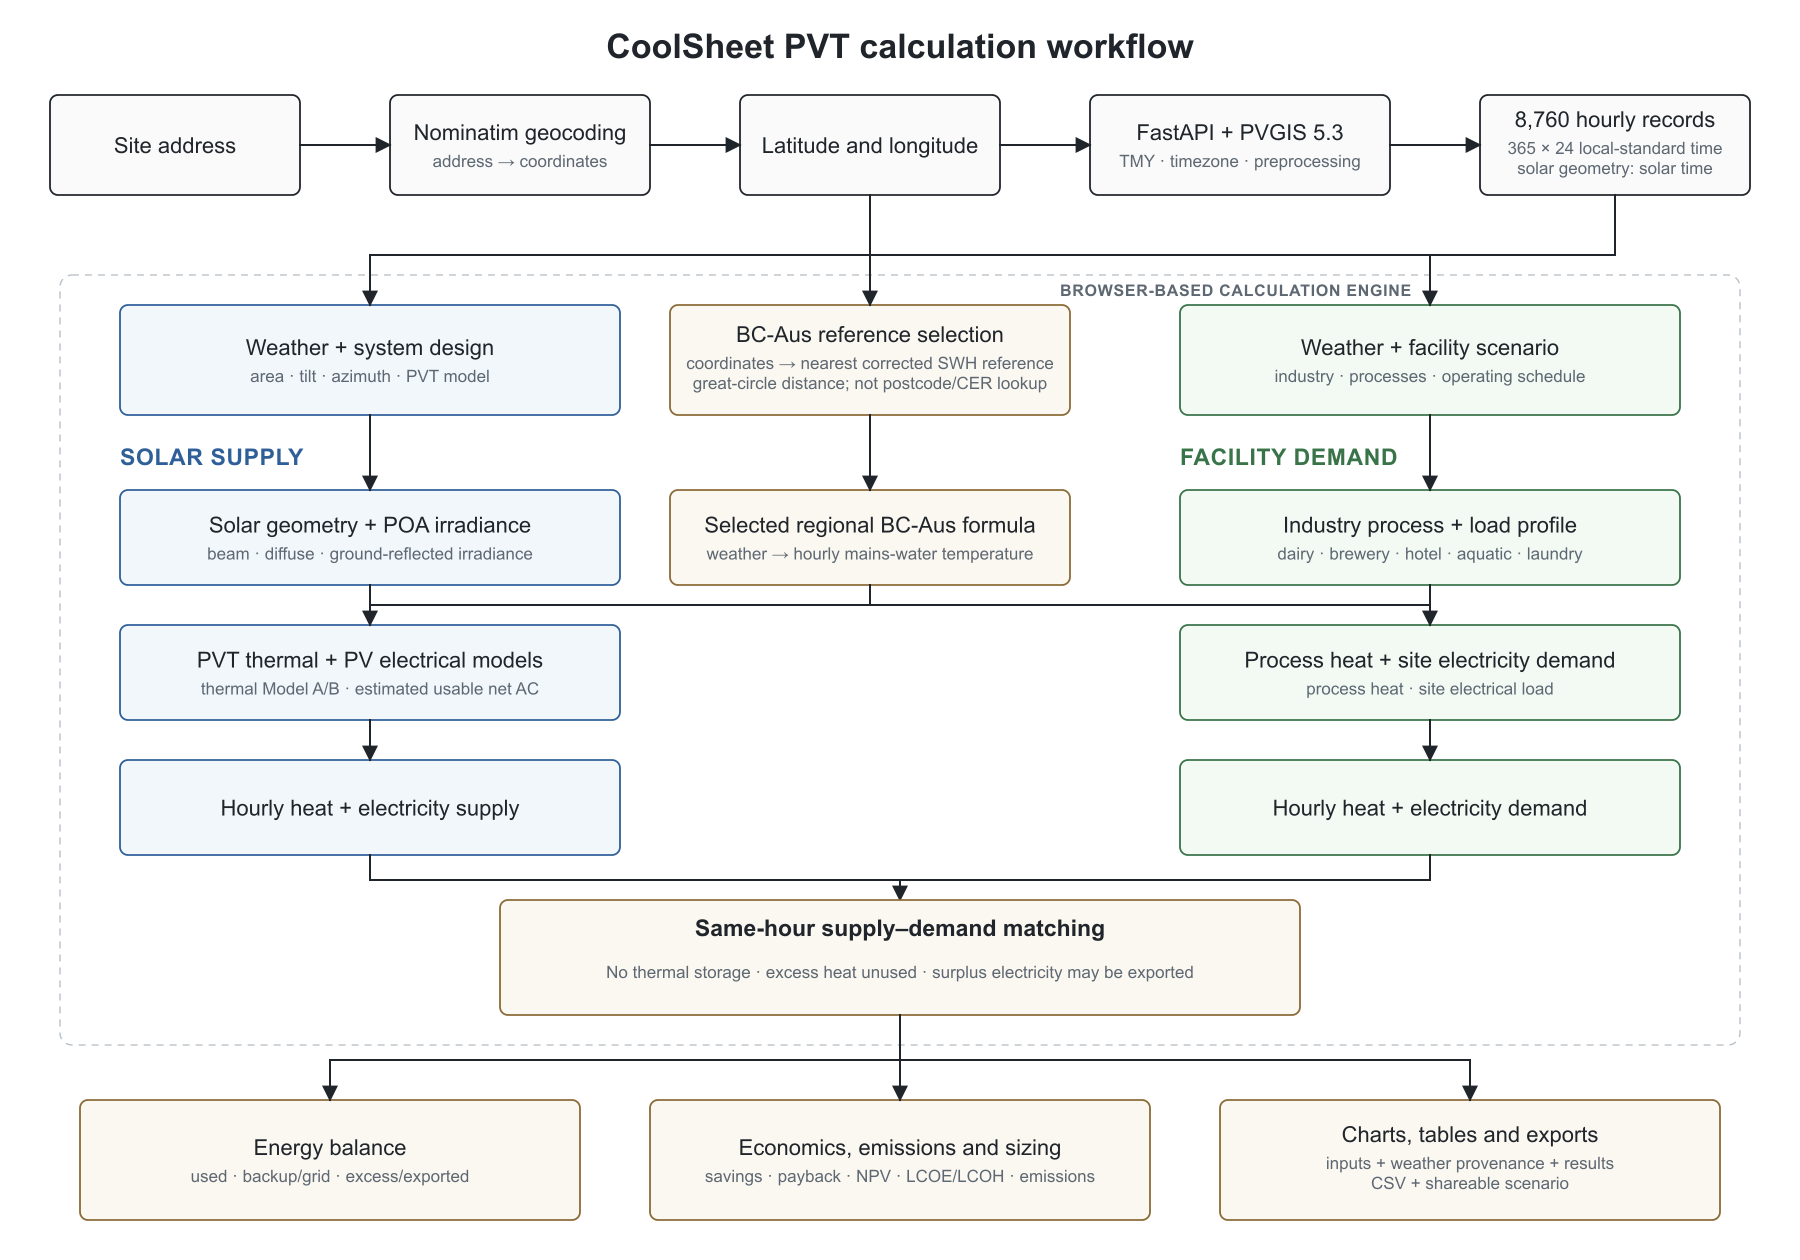
\includegraphics[width=\textwidth]{media/media/PVT Site Workflow.png}
\caption{Overall architecture and hourly calculation workflow of the CoolSheet PVT Calculator. External geocoding and PVGIS weather services support a Python FastAPI backend, while the browser frontend performs all engineering and financial calculations.}
\label{fig:workflow}
\end{figure}

\begin{spacing}{1.27}
Within the browser, the simulation separates into two parallel branches: a supply branch that converts the retrieved weather data into plane-of-array irradiance and then into hourly thermal and alternating-current electrical output (Sections III.D and III.E), and a demand branch that converts facility-scale inputs, process assumptions and operating schedules into hourly thermal and electrical demand for the selected industry (Section III.G).\par

\vspace{0.15in}

The BC-Aus mains-water temperature model, described in Section III.F, provides the shared boundary condition between the two branches.\par

\vspace{0.15in}

The completed supply and demand arrays are then matched independently at each hourly timestep, and the hourly results aggregated into the annual energy, economic and emissions indicators described in Sections III.H--III.J.\par
\end{spacing}

\subsection[User inputs and assumptions\done]{User inputs and assumptions}\label{sec19}

\begin{spacing}{1.27}
User-defined parameters fall into the four categories summarised in Table~\ref{tab:input-groups}, presented in the interface as a site and PVT system panel and an industry demand and economics panel, each with collapsible advanced settings. This structure allows the technical system, facility demand and financial conditions to be varied independently. Default values are provided to permit an initial calculation; however, these defaults represent editable engineering scenarios rather than certified industry benchmarks. Results used for case studies were therefore generated from explicitly stated input sets rather than relying on unspecified interface defaults\textsuperscript{\citenum{37}}. The complete input register, including interface labels, units, shipped defaults and accepted ranges, is provided in Appendix~A.\par
\end{spacing}

\begin{table}[htbp]
\centering
\renewcommand{\thetable}{3}
\small
\begin{tabular}{@{}>{\raggedright\arraybackslash}p{1.7in}>{\raggedright\arraybackslash}p{4.1in}@{}}
\toprule
\textbf{Group} & \textbf{Examples} \\
\midrule
Site and PVT system & Address, area, tilt, azimuth, flow rate and collector coefficients \\
Facility demand & Industry, facility scale, process selections and schedule \\
Economics and emissions & Tariffs, fuel price, boiler efficiency, CAPEX, OPEX and emissions factors \\
Optional overrides & Monthly mains temperatures and editable model parameters \\
\bottomrule
\end{tabular}
\caption{Principal user-input groups of the CoolSheet PVT Calculator.}
\label{tab:input-groups}
\end{table}

\begin{spacing}{1.27}
Several system-level boundaries were fixed to maintain an appropriate level of complexity for preliminary feasibility assessment. The model uses a fixed-tilt homogeneous array and hourly TMY weather\textsuperscript{\citenum{35}}, with site-specific shading, tracking and detailed hydraulic design excluded and wiring, mismatch, soiling and availability effects combined within a single user-defined system-loss factor. Thermal and electrical supply are matched directly to simultaneous demand, with no thermal or battery storage: excess heat is recorded as unused, surplus electricity may be exported, and unmet thermal and electrical demand are assigned to the existing auxiliary heating system and the grid respectively. These boundaries prevent energy generated in one hour from being credited against demand in another, and define the calculator as an early-stage screening model rather than a detailed system-design simulation.\par
\end{spacing}

\subsection[Weather-data acquisition\done]{Weather-data acquisition}\label{sec20}

\begin{spacing}{1.27}
Location-specific weather data were obtained automatically after the user entered a site address. The address was submitted to the OpenStreetMap Nominatim search service and converted into latitude and longitude coordinates, which were retained as the site location for weather retrieval, solar geometry and BC-Aus reference selection\textsuperscript{\citenum{34}}.\par

\vspace{0.15in}

The coordinates were transmitted to the calculator's Python FastAPI backend, which retrieved a Typical Meteorological Year dataset, as defined in Section II.C, from Version 5.3 of the European Commission's Photovoltaic Geographical Information System\textsuperscript{\citenum{35},\citenum{38}} using the \texttt{get\_pvgis\_tmy} function provided by the pvlib Python library\textsuperscript{\citenum{36}}. The implemented request used a fixed source period from 2005 to 2023, preventing the simulated dataset from changing automatically when additional source years become available\textsuperscript{\citenum{37}}.\par

\vspace{0.15in}

For each site, the backend returned 365 days containing 24 hourly records. The principal fields used by the calculator were direct normal irradiance, diffuse horizontal irradiance, global horizontal irradiance, ambient-air temperature and wind speed, together with relative humidity, which is used only by the aquatic-centre outdoor-pool evaporation calculation. Irradiance data provided the inputs to the tilted-surface radiation calculation described in Section III.D, while ambient temperature and wind speed were used by the PVT thermal and electrical models. The ambient-temperature series also supplied the site statistics required by the BC-Aus mains-water temperature model.\par

\vspace{0.15in}

The returned timestamps were converted into a synthetic 365-day local-standard-time calendar, with daylight-saving transitions excluded so that every day retained exactly 24 unique hourly records. A separate true-solar-time field was calculated from the UTC timestamp, site longitude and equation of time, and was used only for solar-position calculations; industry operating schedules continued to use local standard clock time. Separating the two time bases prevented daylight-saving transitions, and the difference between clock time and solar time, from shifting either the solar-resource calculation or the facility load profile\textsuperscript{\citenum{37}}. The complete weather-record structure is listed in Appendix~B.\par
\end{spacing}

\subsection[Solar geometry and irradiance transposition\done]{Solar geometry and irradiance transposition}\label{sec21}

\begin{spacing}{1.27}
The weather dataset provides direct normal irradiance and diffuse horizontal irradiance, whereas the PVT models require the total irradiance incident on the inclined collector surface. Solar geometry and irradiance transposition were therefore evaluated independently for each of the 8,760 hourly weather records, using the site latitude, day of year, true solar time, collector tilt, surface azimuth and ground albedo.\par

\vspace{0.15in}

Solar declination was estimated using the Cooper correlation\textsuperscript{\citenum{39}}, and the hour angle from true solar time:

\begin{align}
\delta &= 23.45 \sin\left[\frac{360}{365}\left(n+284\right)\right], \label{eq:declination}\\
\omega &= 15\left(h_{\mathrm{s}}-12\right), \label{eq:hourangle}
\end{align}

\noindent where $n$ is the day of year and $h_{\mathrm{s}}$ is the true solar hour defined in Section III.C, so that $\omega=0^\circ$ at solar noon.\par

\vspace{0.15in}

The solar zenith angle and the incidence angle between the direct beam and the collector normal follow from the site latitude $\phi$, declination and hour angle\textsuperscript{\citenum{40}}:

\begin{align}
\cos\theta_{\mathrm{z}} ={}& \sin\delta\sin\phi + \cos\delta\cos\phi\cos\omega, \label{eq:zenith}\\
\cos\theta_{\mathrm{i}} ={}& \sin\delta\sin\phi\cos\beta -\sin\delta\cos\phi\sin\beta\cos\gamma_{\mathrm{s}} \notag\\
&+\cos\delta\cos\phi\cos\beta\cos\omega +\cos\delta\sin\phi\sin\beta\cos\gamma_{\mathrm{s}}\cos\omega \notag\\
&+\cos\delta\sin\beta\sin\gamma_{\mathrm{s}}\sin\omega, \label{eq:incidence}
\end{align}

\noindent where $\beta$ is the collector tilt and $\gamma_{\mathrm{s}}$ is the surface azimuth. The interface defines azimuth relative to north over the range $-180^\circ$ to $+180^\circ$ ($0^\circ$ north, $+90^\circ$ east, $\pm180^\circ$ south, $-90^\circ$ west) and subtracts $180^\circ$ internally to obtain $\gamma_{\mathrm{s}}$ in the solar-geometry convention, in which $0^\circ$ is south-facing. The shipped default of $0^\circ$ therefore specifies a north-facing collector, as appropriate for the Southern Hemisphere\textsuperscript{\citenum{37},\citenum{40}}.\par
\end{spacing}

\begin{figure}[!htb]
\centering
\fbox{%
\begin{tikzpicture}[x=0.92cm, y=0.92cm, every node/.style={font=\small}]

% Horizontal reference plane
\draw[dashed, gray!55, thick] (-0.5,0) -- (8.3,0);
\node[gray!40!black, font=\footnotesize, anchor=east] at (8.3,-0.35) {Horizontal reference plane};

% Ground strip (reflective ground in front of collector)
\draw[gray!25, line width=6pt] (2.1,0) -- (4.3,0);
\node[gray!45!black, font=\footnotesize] at (3.2,-0.55) {ground};

% PVT collector
\draw[line width=6pt, gray!35] (2,0) -- (0.3,3.2);
\draw[line width=1.2pt] (2,0) -- (0.3,3.2);
\node[font=\footnotesize, align=center] at (-0.55,3.15) {PVT\\collector};

% Tilt angle beta
\draw[thin] (2,0) -- ++(1.5,0);
\draw[thin] (2.55,0) arc (0:118:0.55);
\node[font=\footnotesize] at (1.9,0.6) {$\beta$};

% Collector normal
\draw[-{Latex[length=2mm]}, thick] (1.15,1.6) -- (3.15,2.65);
\node[font=\footnotesize] at (3.3,2.95) {normal};

% Sun
\draw[fill=yellow!65!orange, draw=orange!70!black] (7.4,6.2) circle (0.28);
\node[font=\small] at (7.75,6.75) {Sun};

% DNI beam
\draw[-{Latex[length=2.5mm]}, orange!70!black, thick] (7.4,6.2) -- (1.15,1.6);
\node[orange!70!black, font=\footnotesize] at (5.2,4.5) {DNI};

% Zenith construction
\coordinate (G) at (6,0);
\draw[dotted, gray!55, thick] (G) -- ++(0,4.3);
\node[gray!40!black, font=\footnotesize] at (6.2,4.4) {zenith};
\draw[gray!50, thin] (G) -- (7.4,6.2);
\draw[gray!40!black, thin] (G) ++(0,0.85) arc (90:75:0.85);
\node[gray!40!black, font=\footnotesize] at (6.85,1.05) {$\theta_{\mathrm{z}}$};

% Incidence angle
\draw[thin] (1.15,1.6) ++(28:0.5) arc (28:38:0.5);
\node[font=\footnotesize] at (2.05,2.3) {$\theta_{\mathrm{i}}$};

% DHI arrows
\draw[-{Latex[length=2mm]}, blue!55!black, thick] (0.15,4.6) -- (0.7,2.5);
\draw[-{Latex[length=2mm]}, blue!55!black, thick] (1.5,4.9) -- (1.25,2.55);
\draw[-{Latex[length=2mm]}, blue!55!black, thick] (2.8,4.3) -- (1.7,2.15);
\node[blue!55!black, font=\footnotesize] at (1.5,4.55) {DHI};

% Ground-reflected arrows
\draw[-{Latex[length=2mm]}, brown!55!black, thick] (4.4,0.05) -- (1.55,1.15);
\draw[-{Latex[length=2mm]}, brown!55!black, thick] (3.6,0.05) -- (1.85,0.85);
\node[brown!55!black, font=\footnotesize, align=center] at (3.5,-1.15) {$G_{\mathrm{r}}$\\(ground-reflected)};

% Component labels
\node[font=\footnotesize] at (0.55,1.3) {$G_{\mathrm{b}}$};
\node[font=\footnotesize] at (1.0,2.9) {$G_{\mathrm{d}}$};

% Total irradiance box
\node[draw, fill=white, rounded corners, font=\footnotesize] at (7.2,-1.15) {$G = G_{\mathrm{b}}+G_{\mathrm{d}}+G_{\mathrm{r}}$};

% phi / gamma note
\node[draw, dashed, gray!45!black, align=left, font=\footnotesize, text width=3.6cm] at (2.2,6.3) {$\phi$ = site latitude\\$\gamma$ = surface azimuth (plan view, not shown)};

\end{tikzpicture}%
}
\caption{Solar geometry and irradiance components used to calculate plane-of-array irradiance on the inclined PVT collector. Direct normal irradiance is projected according to the incidence angle, while diffuse-sky and ground-reflected components are determined using isotropic view factors. The three components are summed to obtain the hourly irradiance supplied to the PVT thermal and electrical models. Source: author.}
\label{fig:solar-geometry}
\end{figure}

\begin{spacing}{1.27}
Total plane-of-array irradiance was calculated using an isotropic diffuse-sky model\textsuperscript{\citenum{41}}. The horizontal beam component, reconstructed global horizontal irradiance and the three components incident on the tilted collector were obtained from

\begin{align}
G_{\mathrm{BHI}} &= \mathrm{DNI}\max\left(0,\cos\theta_{\mathrm{z}}\right), \label{eq:gbhi}\\
G_{\mathrm{HI}} &= G_{\mathrm{BHI}}+\mathrm{DHI}, \label{eq:ghi}\\
G_{\mathrm{b}} &= \mathrm{DNI}\max\left(0,\cos\theta_{\mathrm{i}}\right), \label{eq:gb}\\
G_{\mathrm{d}} &= \mathrm{DHI}\left(\frac{1+\cos\beta}{2}\right), \label{eq:gd}\\
G_{\mathrm{r}} &= G_{\mathrm{HI}}\,\rho_{\mathrm{g}}\left(\frac{1-\cos\beta}{2}\right), \label{eq:gr}\\
G &= \max\left(0,\, G_{\mathrm{b}}+G_{\mathrm{d}}+G_{\mathrm{r}}\right), \label{eq:gtotal}
\end{align}

\noindent where $\rho_{\mathrm{g}}$ is the ground albedo. Direct irradiance was set to zero when the sun was below the horizon or behind the collector plane, and negative irradiance inputs were prevented from propagating through the calculation.\par

\vspace{0.15in}

The isotropic model assumes uniform diffuse-sky irradiance and therefore omits circumsolar and horizon-brightening effects. It was retained as the production transposition method because it is transparent, computationally efficient and consistent with the irradiance basis used by the implemented PVT models\textsuperscript{\citenum{37},\citenum{41}}.\par
\end{spacing}

\subsection[PVT supply model\done]{PVT supply model}\label{sec22}

\begin{spacing}{1.27}
The PVT supply model converted the hourly plane-of-array irradiance $G$ calculated in Section III.D, together with ambient-air temperature $T_{\mathrm{a}}$, wind speed $u$, mains-water inlet temperature $T_{\mathrm{in}}$, collector area $A$ and heat-transfer-fluid flow rate, into hourly useful thermal energy, outlet-fluid temperature, PVT electrical energy and a conventional PV-only electrical baseline.\par

\vspace{0.15in}

\textbf{Thermal output.} Two alternative thermal formulations were implemented. Model A was retained as a project-specific inlet-temperature correlation, whereas Model B applied the ISO 9806 collector-performance formulation\textsuperscript{\citenum{37},\citenum{42}}. The coefficient sets are model-specific and were not interchanged because Model A uses inlet-fluid temperature while Model B uses mean-fluid temperature. Full-precision coefficients for both models are listed in Appendix~A. For Model A, hourly thermal efficiency and useful thermal power were

\begin{align}
\eta_{\mathrm{th,A}} &= \mathrm{clamp}\left[a_{0,\mathrm{A}} + a_{1,\mathrm{A}}\left(\frac{T_{\mathrm{in}}-T_{\mathrm{a}}}{G}\right) + a_{2,\mathrm{A}}u,\; 0,\; 1\right], \label{eq:etaA}\\
\dot{Q}_{\mathrm{th}} &= \eta_{\mathrm{th,A}}\,G\,A, \label{eq:qthA}
\end{align}

\noindent where $a_{0,\mathrm{A}}$ is the zero-loss coefficient, $a_{1,\mathrm{A}}$ represents the inlet-temperature loss dependence and $a_{2,\mathrm{A}}$ represents the wind-speed dependence. Efficiency and useful power were set to zero when irradiance was negligible.\par

\vspace{0.15in}

Model B used the mean fluid temperature $T_{\mathrm{m}}=\left(T_{\mathrm{in}}+T_{\mathrm{out}}\right)/2$. In the production configuration the optional wind and long-wave coefficients are zero, so the implemented ISO 9806 relation reduces to the quadratic steady-state form\textsuperscript{\citenum{42}}:

\begin{equation}
\dot{Q}_{\mathrm{th}} = A\left[\eta_0 G - a_1\left(T_{\mathrm{m}}-T_{\mathrm{a}}\right) - a_2\left(T_{\mathrm{m}}-T_{\mathrm{a}}\right)^2\right],
\label{eq:qthB}
\end{equation}

\noindent where $\eta_0$ is the zero-loss efficiency and $a_1$ and $a_2$ are the linear and quadratic heat-loss coefficients. The remaining ISO 9806 terms are retained within the software so that alternative certified coefficient sets can be applied.\par

\vspace{0.15in}

Because $T_{\mathrm{out}}$ appears within the mean-fluid temperature, Model B was solved iteratively from the fluid energy balance

\begin{equation}
\dot{m}c_p\left(T_{\mathrm{out}}-T_{\mathrm{in}}\right) - \dot{Q}_{\mathrm{th}}\left(T_{\mathrm{out}}\right) = 0,
\label{eq:energybalance}
\end{equation}

\noindent using Newton--Raphson iteration, with the solver configuration reported in Appendix~A\textsuperscript{\citenum{37}}. For Model A, the outlet temperature was calculated directly from the same balance after useful thermal power had been determined. Negative useful thermal power was set to zero for both models.\par

\begin{figure}[!htb]
\centering
\fbox{%
\begin{tikzpicture}[x=1cm, y=1cm, every node/.style={font=\small}]

% Ambient conditions
\node[blue!55!black, font=\footnotesize, align=center] at (12.4,7.45) {Ambient air\\$T_{\mathrm{a}}$, wind $u$};

% Incident plane-of-array irradiance
\foreach \x in {3.4,4.6,5.8}{%
  \draw[-{Latex[length=2mm]}, orange!70!black, thick] (\x,7.05) -- ++(0.8,-2.15);
}
\node[orange!70!black, font=\footnotesize, align=center] at (3.1,7.55) {Plane-of-array\\irradiance $G$};

% Combined thermal loss to ambient
\draw[-{Latex[length=2mm]}, blue!55!black, thick] (8.5,4.95) -- ++(-0.4,1.75);
\draw[-{Latex[length=2mm]}, blue!55!black, thick] (9.4,4.95) -- ++(0.4,1.75);
\node[blue!55!black, font=\footnotesize, align=center] at (8.6,7.35) {Thermal loss to ambient\\$a_1(T_{\mathrm{m}}-T_{\mathrm{a}})+a_2(T_{\mathrm{m}}-T_{\mathrm{a}})^2$};

% Control volume
\draw[dashed, gray!60] (2.9,2.7) rectangle (10.3,5.0);
\node[gray!45!black, font=\footnotesize, anchor=north] at (6.6,2.62) {Collector control volume, aperture area $A$};

\fill[gray!30] (3.15,4.25) rectangle (10.05,4.85);
\draw[line width=0.9pt] (3.15,4.25) rectangle (10.05,4.85);
\node[font=\footnotesize] at (6.6,4.55) {PV laminate, cell temperature $T_{\mathrm{cell,PVT}}$};

\fill[blue!10] (3.15,3.0) rectangle (10.05,4.25);
\draw[line width=0.9pt] (3.15,3.0) rectangle (10.05,4.25);
\node[font=\footnotesize, align=center] at (6.6,3.62) {Absorber and fluid channel\\mean fluid temperature $T_{\mathrm{m}}$};

% Fluid inlet and outlet
\draw[-{Latex[length=2mm]}, green!35!black, thick] (1.5,3.55) -- (3.1,3.55);
\node[green!35!black, font=\footnotesize, align=center, anchor=east] at (1.45,3.55) {$\dot m$, $c_p$\\$T_{\mathrm{in}}$};
\draw[-{Latex[length=2mm]}, green!35!black, thick] (10.1,3.55) -- (11.7,3.55);
\node[green!35!black, font=\footnotesize, anchor=west] at (11.75,3.55) {$T_{\mathrm{out}}$};

% Direct-current electrical output
\draw[-{Latex[length=2mm]}, red!55!black, thick] (10.1,4.55) -- (11.7,5.35);
\node[red!55!black, font=\footnotesize, anchor=west] at (11.75,5.45) {$E_{\mathrm{DC}}$};

% Resulting quantities
\draw[-{Latex[length=2mm]}, gray!55] (3.4,2.67) -- (3.4,2.18);
\draw[-{Latex[length=2mm]}, gray!55] (9.9,2.67) -- (10.4,2.18);

\node[draw, rounded corners, fill=white, font=\footnotesize, align=center, text width=4.0cm]
  at (3.6,1.45) {\textbf{Useful thermal}\\[1pt]$\dot Q_{\mathrm{th}} = \dot m c_p\left(T_{\mathrm{out}}-T_{\mathrm{in}}\right)$};
\node[draw, rounded corners, fill=white, font=\footnotesize, align=center, text width=5.6cm]
  at (10.4,1.45) {\textbf{Net electrical}\\[1pt]$E_{\mathrm{DC}} = E_{\mathrm{ref}}f_T\!\left(T_{\mathrm{cell,PVT}}\right)$,\quad $E_{\mathrm{AC}} = E_{\mathrm{DC}}\left(1-L_{\mathrm{sys}}\right)\eta_{\mathrm{inv}}$};

% Coupling between the two branches
\draw[-{Latex[length=2mm]}, dashed, gray!55!black, thick] (5.75,1.45) -- (7.35,1.45);
\node[gray!45!black, font=\footnotesize, align=center] at (6.55,0.35) {Heat extraction $\dot Q_{\mathrm{cool}}/(U_{\mathrm{L}}A)$\\lowers the cell temperature};

\end{tikzpicture}%
}
\caption{Energy balance of the PVT collector control volume. Plane-of-array irradiance is absorbed at the aperture; part is carried away by the heat-transfer fluid between inlet and outlet, part is lost to ambient through the lumped loss coefficients, and the remainder leaves the PV laminate as direct-current electricity. Losses are shown as a single combined term because both thermal formulations lump them into fitted coefficients; the separate wind and long-wave terms of ISO 9806 are implemented but zero in the production configuration. Heat extraction lowers the cell temperature, which is the only coupling between the thermal and electrical branches.}
\label{fig:pvt-balance}
\end{figure}

\vspace{0.15in}

\textbf{Electrical output.} The reference electrical energy available in each timestep and the uncooled PV cell temperature were calculated as\textsuperscript{\citenum{40},\citenum{43}}

\begin{align}
E_{\mathrm{ref}} &= \frac{\eta_{\mathrm{PV}}\,G\,A\,\Delta t}{1000}, \label{eq:eref}\\
T_{\mathrm{cell,PV}} &= T_{\mathrm{a}} + \frac{G}{800}\left(T_{\mathrm{NOCT}}-20\right), \label{eq:tcellpv}
\end{align}

\noindent where $\eta_{\mathrm{PV}}$ is the module efficiency at standard test conditions, $\Delta t=1$~h and $T_{\mathrm{NOCT}}$ is the nominal operating cell temperature. A separate PVT cell temperature represented cooling caused by thermal energy extraction:

\begin{equation}
T_{\mathrm{cell,PVT}} = \mathrm{clamp}\left[T_{\mathrm{cell,PV}} - \frac{\dot{Q}_{\mathrm{cool}}}{U_{\mathrm{L}}A},\; T_{\mathrm{in}},\; T_{\mathrm{cell,PV}}\right],
\label{eq:tcellpvt}
\end{equation}

\noindent where $\dot{Q}_{\mathrm{cool}} = \dot{m}c_p\left(T_{\mathrm{out}}-T_{\mathrm{in}}\right)$ and $U_{\mathrm{L}}$ is the absolute first-order heat-loss coefficient of the active thermal model\textsuperscript{\citenum{37}}.\par

\vspace{0.15in}

The temperature-dependent correction and the conversion to net alternating-current energy were

\begin{align}
f_T &= \max\left[0,\; 1+\gamma_{\mathrm{P}}\left(T_{\mathrm{cell}}-25\right)\right], \label{eq:ftemp}\\
E_{\mathrm{DC,PVT}} &= E_{\mathrm{ref}}\,f_T\!\left(T_{\mathrm{cell,PVT}}\right), \quad E_{\mathrm{DC,PV}} = E_{\mathrm{ref}}\,f_T\!\left(T_{\mathrm{cell,PV}}\right), \label{eq:edc}\\
E_{\mathrm{AC}} &= E_{\mathrm{DC}}\left(1-L_{\mathrm{sys}}\right)\eta_{\mathrm{inv}}, \label{eq:eac}
\end{align}

\noindent where $\gamma_{\mathrm{P}}$ is the module power-temperature coefficient, $L_{\mathrm{sys}}$ is the combined non-inverter direct-current loss fraction and $\eta_{\mathrm{inv}}$ is the inverter efficiency. Net alternating-current PVT energy was used for the reported electricity generation, hourly demand matching and economic calculations, while the PV-only result was retained as a reference for the estimated electrical effect of thermal cooling.\par

\vspace{0.15in}

The cooling relationship is a bounded sensitivity model rather than a detailed cell--absorber heat-transfer model. It was not treated as independently field-validated, and it can be disabled so that PVT and PV-only electrical production are identical. Figure~\ref{fig:pvt-balance} summarises the resulting control volume and the coupling between the two branches.\par
\end{spacing}


\subsection[Australian mains-water temperature model\done]{Australian mains-water temperature model}\label{sec23}

\begin{spacing}{1.27}
A location-responsive mains-water temperature model was developed because incoming water temperature affects both sides of the PVT assessment. It provides the collector inlet-temperature condition used in the thermal supply model and the initial water temperature used to calculate process-heating demand. A single constant value would therefore introduce the same climatic simplification into both the predicted supply and the facility demand.\par

\vspace{0.15in}

\textbf{Model formulation.} The BC-Aus model retained the sinusoidal structure of the original Burch--Christensen relationship. For each day of the representative year, the mains-water temperature is calculated as:

\begin{equation}
T_{\mathrm{mains,F}}(d) = \left(T_{\mathrm{a,F}} + C_{\mathrm{off}}\right) + R\left(\frac{\Delta T_{\mathrm{a,F}}}{2}\right)\sin\left[0.986\left(d_m - 15 - L\right) - 90^\circ\right]
\label{eq:bcaus}
\end{equation}

\noindent where:
\begin{itemize}
  \item $T_{\mathrm{mains,F}}(d)$ is the predicted daily mains-water temperature in $^\circ$F;
  \item $T_{\mathrm{a,F}}$ is the annual mean ambient-air temperature;
  \item $\Delta T_{\mathrm{a,F}}$ is the difference between the warmest and coolest monthly mean ambient temperatures;
  \item $C_{\mathrm{off}}$ is the mean-temperature offset;
  \item $R$ is the seasonal amplitude ratio;
  \item $L$ is the phase lag in days;
  \item $d_m$ is the hemisphere-adjusted model day.
\end{itemize}

The equation is evaluated in the original Fahrenheit domain and the resulting values are converted to degrees Celsius. The original Building America implementation used an offset of $+6^\circ$F and climate-dependent expressions for amplitude and lag.\par

\vspace{0.15in}

\textbf{Southern Hemisphere adaptation.} The original calendar convention follows Northern Hemisphere seasonality. For Australian locations, the model day was shifted by approximately half a year:

\begin{equation}
d_m = \left(\left(d + 181\right) \bmod 365\right) + 1
\label{eq:daymodel}
\end{equation}

\noindent where $d$ is the calendar day of year. The shift is applied only to sites at southern latitudes; it sets the broad seasonal orientation, while the fitted phase lag provides the smaller location-specific timing adjustment.\par

\vspace{0.15in}

\textbf{Australian reference fitting.} Monthly cold-water reference values were obtained from five legacy Clean Energy Regulator domestic simulation decks associated with Rockhampton, Alice Springs, Sydney, Melbourne and Canberra. These values are Australian simulation references rather than measured utility mains-water records, and this distinction governs how the model's agreement statistics must be interpreted in Section IV.B. National fits retaining or removing the original fixed offset could not reproduce differences in seasonal amplitude and timing between the reference climates, so each reference profile was instead fitted separately using three effective parameters: mean-temperature offset, amplitude ratio and phase lag. A deterministic three-parameter procedure was adopted because an earlier five-parameter formulation was rank-deficient for a single fixed ambient series and produced model-equivalent but platform-dependent coefficient sets. The complete fitting derivation, data lineage and the excluded Canberra parameters are provided in the appendix.
\end{spacing}

\begin{table}[htbp]
\centering
\renewcommand{\thetable}{4}
\begin{tabular}{@{}lccc@{}}
\toprule
\textbf{Reference location} & \textbf{Offset ($^\circ$F)} & \textbf{Amplitude ratio} & \textbf{Phase lag (days)} \\
\midrule
Rockhampton   & $+5.424$ & 0.802 & $-6.740$ \\
Alice Springs & $-0.473$ & 1.061 & $-8.622$ \\
Sydney        & $-0.377$ & 1.034 & $-0.086$ \\
Melbourne     & $-0.822$ & 0.973 & $+0.701$ \\
\bottomrule
\end{tabular}
\caption{Fitted BC-Aus coefficients used for runtime reference selection.}
\label{tab:bcaus-coeffs}
\end{table}

\begin{spacing}{1.27}
The original $+6^\circ$F offset remained approximately appropriate only for Rockhampton, while the fitted offsets for the remaining references were close to zero (Table~\ref{tab:bcaus-coeffs}).\par

\vspace{0.15in}

\textbf{Location-based runtime calculation.} When a user enters an address, the geocoded coordinates are compared with the four runtime reference locations and the geographically nearest is selected using the haversine distance, applying its fitted offset, amplitude ratio and phase lag. This is a nearest-reference engineering approximation rather than an official CER postcode-zone determination. The selected reference and its distance from the site are retained in the result object, but are shown on screen only when the interface's diagnostic mode is enabled.\par

\vspace{0.15in}

The selected coefficients are combined with climate statistics calculated from the PVGIS Typical Meteorological Year dataset for the actual user-selected site, which supplies the annual mean ambient temperature and the warmest-to-coolest monthly temperature range. Consequently, a site assigned to the Melbourne reference does not simply receive Melbourne's stored monthly profile; the Melbourne-fitted relationship is applied using the actual site's climate statistics.
\end{spacing}

\begin{spacing}{1.27}
\textbf{Integration with the calculator.} The BC-Aus output contains one temperature for each of the 365 days in the representative year. Each daily value is applied to the corresponding hourly records in the 8,760-hour simulation. Within the PVT thermal model, it defines the collector inlet temperature. Within the industry models, the sensible energy required to heat incoming water is calculated using:

\begin{equation}
Q_{\mathrm{water}} = m_{\mathrm{water}}\, c_p\, \max\left(0,\, T_{\mathrm{target}} - T_{\mathrm{mains}}\right)
\label{eq:qwater}
\end{equation}

The daily profile is used in the dairy, brewery and commercial-laundry water-heating calculations and in aquatic-centre makeup-water heating. Users may replace the automatically generated profile by entering twelve monthly mains-water temperatures where measured or preferred site data are available; months left blank fall back to the modelled daily value.
\end{spacing}

\subsection{Industry-demand models}\label{sec24}

\begin{spacing}{1.27}
The industry-demand models converted annual facility activity into separate hourly thermal and electrical demand profiles. For each industry, annual demand was first estimated from a physical activity variable, such as product throughput, occupancy or water-surface area. Normalised monthly and hourly weighting factors were then applied to distribute this demand across the 8,760-hour representative year.\par

\vspace{0.15in}

For water-heating processes, the hourly thermal demand was calculated from the volume of water used, the daily mains-water temperature and the required process temperature:

\begin{equation}
Q_{p,h} = \frac{V_{p,h}\,\rho_{\mathrm{w}}\,c_p\max\left(0,\,T_{p,\mathrm{target}}-T_{\mathrm{mains},h}\right)}{3600},
\label{eq:qprocess}
\end{equation}

\noindent where $Q_{p,h}$ is the thermal demand of process $p$ during hour $h$ in kWh, $V_{p,h}$ is the corresponding water volume in litres, $\rho_{\mathrm{w}}=1$~kg\,L$^{-1}$ and $c_p=4.184$~kJ\,kg$^{-1}$\,K$^{-1}$. The zero bound prevents negative heating demand when the mains-water temperature exceeds the selected preheating target.\par
\end{spacing}

\subsubsection[Dairy\done]{Dairy}\label{sec25}

\begin{spacing}{1.27}
The dairy model represents a dairy-farm or dairy-shed operating scenario rather than a complete milk-processing factory. It estimates electricity use associated with milking, milk cooling, refrigeration, pumping and cleaning, together with low-temperature water preheating for three selectable thermal processes. Pasteurisation, homogenisation, evaporation, drying and other large-scale manufacturing loads are outside the model boundary.\par
\end{spacing}

\begin{figure}[!htb]
\centering
\fbox{%
\begin{tikzpicture}[
  tbox/.style={rectangle, draw=orange!55!black, rounded corners, fill=orange!6, align=center,
    text width=2.4cm, minimum height=0.95cm, font=\scriptsize, inner sep=3pt,
    execute at begin node={\hyphenpenalty=10000\relax}},
  ebox/.style={rectangle, draw=blue!45!black, rounded corners, fill=blue!5, align=center,
    text width=2.4cm, minimum height=0.95cm, font=\scriptsize, inner sep=3pt,
    execute at begin node={\hyphenpenalty=10000\relax}},
  src/.style={rectangle, draw=gray!55, rounded corners, fill=gray!8, align=center,
    text width=2.2cm, minimum height=0.95cm, font=\scriptsize, inner sep=3pt,
    execute at begin node={\hyphenpenalty=10000\relax}},
  outbox/.style={rectangle, draw=green!25!black, rounded corners, fill=green!45!black, text=white,
    align=center, text width=3.0cm, minimum height=0.95cm, font=\bfseries\scriptsize, inner sep=3pt,
    execute at begin node={\hyphenpenalty=10000\relax}},
  arr/.style={-{Latex[length=1.8mm]}, thick, draw=gray!50!black},
  lbl/.style={font=\bfseries\scriptsize, align=left}
]

\node[src] (milk) at (0,0) {Annual milk throughput};

% thermal pathway
\node[lbl, text=orange!60!black] at (3.9,1.75) {THERMAL PATHWAY};
\node[tbox] (t1) at (3.9,1.05) {Process-water coefficients};
\node[tbox] (t2) at (6.9,1.05) {Seasonal and hourly schedules};
\node[tbox] (t3) at (9.9,1.05) {Daily BC-Aus mains temperature};

% electrical pathway
\node[lbl, text=blue!55!black] at (3.9,-0.5) {ELECTRICAL PATHWAY};
\node[ebox] (e1) at (3.9,-1.2) {Electricity intensity};
\node[ebox] (e2) at (6.9,-1.2) {Seasonal and milking-period weighting};

\node[outbox] (o) at (12.6,-0.1) {8,760-hour thermal and electrical demand};

\draw[arr] (milk.east) |- (t1.west);
\draw[arr] (t1) -- (t2);
\draw[arr] (t2) -- (t3);
\draw[arr] (milk.east) |- (e1.west);
\draw[arr] (e1) -- (e2);
\draw[arr] (t3.east) -| (o.north);
\draw[arr] (e2.east) -| (o.south);

\end{tikzpicture}%
}
\caption{Construction of the dairy thermal and electrical demand profiles. Annual milk throughput is converted into process-water and electricity requirements, distributed using normalised seasonal and hourly factors, and combined with daily mains-water temperature to generate 8,760-hour demand arrays.}
\label{fig:dairy-demand}
\end{figure}

\begin{spacing}{1.27}
Annual raw-milk throughput was used as the principal activity variable. For thermal process $p$, the annual process-water requirement and its hourly distribution were

\begin{align}
V_{p,\mathrm{annual}} &= V_{\mathrm{milk}}k_p, \label{eq:vpannual}\\
V_{p,h} &= \frac{V_{\mathrm{milk}}k_p}{365}s_m w_{p,h}, \label{eq:vph}
\end{align}

\noindent where $V_{\mathrm{milk}}$ is the annual milk throughput in litres, $k_p$ is the process-water coefficient in litres of water per litre of milk, $s_m$ is the normalised seasonal factor for month $m$ and $w_{p,h}$ is the normalised hourly process weighting. The hourly factors for each process sum to unity over a day, while the monthly factors are normalised according to the number of days in each month:

\begin{equation}
\sum_{h=0}^{23}w_{p,h} = 1, \qquad \sum_{m=1}^{12}D_m s_m = 365,
\label{eq:normfactors}
\end{equation}

\noindent where $D_m$ is the number of days in month $m$. These conditions ensure that the annual process-water volume remains equal to $V_{\mathrm{milk}}k_p$ despite the imposed seasonal and hourly variation\textsuperscript{\citenum{37}}. The three implemented thermal processes are summarised in Table~\ref{tab:dairy-processes}.\par
\end{spacing}

\begin{table}[!htb]
\centering
\renewcommand{\thetable}{5}
\footnotesize
\begin{tabular}{@{}>{\raggedright\arraybackslash}p{1.5in}>{\raggedright\arraybackslash}p{1.25in}>{\raggedright\arraybackslash}p{0.95in}>{\raggedright\arraybackslash}p{1.85in}@{}}
\toprule
\textbf{Process} & \textbf{Water-use coefficient} & \textbf{PVT preheating target} & \textbf{Hourly allocation} \\
\midrule
Fatty-film rinse & 0.30 L\,L$^{-1}$ milk & 35~$^\circ$C & 50\% at 07:00 and 50\% at 17:00 \\
CIP preheating & 0.57 L\,L$^{-1}$ milk & 35~$^\circ$C & 25\% at 08:00, 09:00, 17:00 and 18:00 \\
Boiler-feedwater preheating & 0.50 L\,L$^{-1}$ milk & 35~$^\circ$C & Uniformly distributed across 24 hours \\
\bottomrule
\end{tabular}
\caption{Default process-water coefficients, preheating targets and hourly schedules used in the dairy-demand model.}
\label{tab:dairy-processes}
\end{table}

\begin{spacing}{1.27}
When all three processes were selected, the default annual heated-water requirement was $k_{\mathrm{total}}=0.30+0.57+0.50=1.37$~L\,L$^{-1}$ milk. The 35~$^\circ$C target is a single editable input applied to all three processes, and represents the low-temperature preheating contribution that may be supplied directly by the PVT system. It does not represent the final temperature required for full cleaning-in-place or boiler operation, which would normally require additional auxiliary heating.\par

\vspace{0.15in}

The raw dairy seasonal factors applied from January to December were 0.85, 0.80, 0.85, 0.90, 0.85, 0.75, 0.75, 0.80, 1.10, 1.30, 1.30 and 1.05, producing lower assumed milk activity during winter and a higher production period during spring. Annual thermal energy was not fixed by the normalisation in Eq.~\ref{eq:normfactors} because the daily temperature rise depended on the BC-Aus mains-water profile.\par

\vspace{0.15in}

The annual and hourly dairy electrical demand were calculated as

\begin{align}
E_{\mathrm{el,annual}} &= e_{\mathrm{dairy}}\frac{V_{\mathrm{milk}}}{1000}, \label{eq:eldairyannual}\\
E_{\mathrm{el},h} &= \frac{e_{\mathrm{dairy}}V_{\mathrm{milk}}}{365\,000}s_m w_{\mathrm{el},h}, \label{eq:eldairyh}
\end{align}

\noindent where $e_{\mathrm{dairy}}$ is the electricity intensity in kWh per kilolitre of milk. The default electricity intensity was 51.7~kWh\,kL$^{-1}$, which is within the range reported by Australian dairy-energy audits and close to their reported average\textsuperscript{\citenum{47},\citenum{48}}. The hourly profile contains a low overnight baseload and elevated demand around the assumed morning and afternoon milking periods, approximately 05:00--07:00 and 15:00--17:00, and represents the combined use of the equipment listed above rather than separate appliance-level simulations. A worked example running from milk throughput through to levelised cost is given in Appendix~C.\par

\vspace{0.15in}

The dairy model operates continuously across all days of the year. It should therefore be interpreted as a transparent and editable early-stage scenario rather than a certified facility forecast. The electricity intensity is supported by public Australian benchmark evidence, whereas the exact process-water coefficients and operating schedules remain engineering assumptions based principally on internal project information\textsuperscript{\citenum{37}}. Site-specific assessments should replace these defaults with measured milk throughput, water consumption, operating schedules and interval electricity data where available.\par
\end{spacing}

\subsubsection{Brewery}\label{sec26}

\subsubsection{Hotel}\label{sec27}

\subsubsection{Aquatic centre}\label{sec28}

\subsubsection{Commercial laundry}\label{sec29}

\subsection[Hourly energy matching\done]{Hourly energy matching}\label{sec30}

\begin{spacing}{1.27}
Hourly energy matching was used to determine how much of the predicted PVT output could be used directly by the selected facility. Separate 8,760-value arrays were generated for thermal supply, electrical supply, thermal demand and electrical demand, and supply and demand were compared independently within each hourly timestep. For either the thermal or electrical energy stream $x$, the directly matched energy, unmet demand and excess supply during hour $h$ were

\begin{align}
E_{\mathrm{matched},x,h} &= \min\left(E_{\mathrm{supply},x,h},\; E_{\mathrm{demand},x,h}\right), \label{eq:matched}\\
E_{\mathrm{unmet},x,h} &= \max\left(0,\; E_{\mathrm{demand},x,h}-E_{\mathrm{supply},x,h}\right), \label{eq:unmet}\\
E_{\mathrm{excess},x,h} &= \max\left(0,\; E_{\mathrm{supply},x,h}-E_{\mathrm{demand},x,h}\right), \label{eq:excess}
\end{align}

\noindent which maintain the hourly energy balances $E_{\mathrm{supply},x,h}=E_{\mathrm{matched},x,h}+E_{\mathrm{excess},x,h}$ and $E_{\mathrm{demand},x,h}=E_{\mathrm{matched},x,h}+E_{\mathrm{unmet},x,h}$.\par
\end{spacing}

\begin{figure}[!htb]
\centering
\fbox{%
\begin{tikzpicture}[x=0.28cm, y=0.23cm, font=\footnotesize,
  supplyline/.style={blue!55!black, thick},
  demandline/.style={green!35!black, thick}]

% ---------------- Panel (a): thermal ----------------
\begin{scope}
  \fill[green!12] (2,0) rectangle (7,9);
  \fill[green!12] (12,0) rectangle (17,10);

  % matched = min(supply, demand): clip to each demand block, fill under the supply curve
  \begin{scope}
    \clip (2,0) rectangle (7,9);
    \fill[orange!35] (4,0) -- plot[domain=4:16, samples=60, smooth, variable=\x]
      ({\x},{11.5*sin(180*(\x-4)/12)}) -- (16,0) -- cycle;
  \end{scope}
  \begin{scope}
    \clip (12,0) rectangle (17,10);
    \fill[orange!35] (4,0) -- plot[domain=4:16, samples=60, smooth, variable=\x]
      ({\x},{11.5*sin(180*(\x-4)/12)}) -- (16,0) -- cycle;
  \end{scope}

  \draw[demandline] (0,0) -- (2,0) -- (2,9) -- (7,9) -- (7,0) -- (12,0) -- (12,10) -- (17,10) -- (17,0) -- (20,0);
  \draw[supplyline, domain=4:16, samples=60, smooth, variable=\x]
    plot ({\x},{11.5*sin(180*(\x-4)/12)});

  \draw[-{Latex[length=2mm]}, thick] (-0.5,0) -- (19.5,0) node[below, font=\scriptsize] {hour};
  \draw[-{Latex[length=2mm]}, thick] (0,-0.5) -- (0,15) node[above, font=\scriptsize] {energy};

  \node[font=\scriptsize\bfseries] at (10,16.6) {(a) Thermal};
  \node[orange!60!black, font=\scriptsize, align=center] at (5.0,3.0) {directly\\matched heat};
  \node[green!35!black, font=\scriptsize, align=center] at (3.4,13.8) {auxiliary heating};
  \draw[green!35!black, -{Latex[length=1.5mm]}] (3.0,12.9) -- (2.8,9.4);
  \node[blue!55!black, font=\scriptsize, align=center] at (13.2,13.8) {unused excess heat};
  \draw[blue!55!black, -{Latex[length=1.5mm]}] (12.0,12.9) -- (9.7,8.6);
  \node[gray!45!black, font=\scriptsize] at (10,-2.6) {no transfer to later hours};
\end{scope}

% ---------------- Panel (b): electrical ----------------
\begin{scope}[xshift=7.2cm]
  \fill[green!12] (3,0) rectangle (18,7);

  \begin{scope}
    \clip (3,0) rectangle (18,7);
    \fill[orange!35] (4,0) -- plot[domain=4:16, samples=60, smooth, variable=\x]
      ({\x},{11.5*sin(180*(\x-4)/12)}) -- (16,0) -- cycle;
  \end{scope}

  \draw[demandline] (0,0) -- (3,0) -- (3,7) -- (18,7) -- (18,0) -- (20,0);
  \draw[supplyline, domain=4:16, samples=60, smooth, variable=\x]
    plot ({\x},{11.5*sin(180*(\x-4)/12)});

  \draw[-{Latex[length=2mm]}, thick] (-0.5,0) -- (19.5,0) node[below, font=\scriptsize] {hour};
  \draw[-{Latex[length=2mm]}, thick] (0,-0.5) -- (0,15) node[above, font=\scriptsize] {energy};

  \node[font=\scriptsize\bfseries] at (10,16.6) {(b) Electrical};
  \node[orange!60!black, font=\scriptsize, align=center] at (10,3.0) {on-site\\electricity use};
  \node[blue!55!black, font=\scriptsize] at (10.2,13.4) {grid export};
  \draw[blue!55!black, -{Latex[length=1.5mm]}] (10.2,12.4) -- (10.0,11.2);
  \node[green!35!black, font=\scriptsize, align=center] at (19.6,10.0) {grid\\import};
  \draw[green!35!black, -{Latex[length=1.5mm]}] (19.6,8.8) -- (17.4,6.6);
\end{scope}

\end{tikzpicture}%
}
\caption{Hourly matching of PVT supply and facility demand over a representative day. In each timestep the overlap between supply and demand is recorded as directly utilised energy; unmet thermal demand is supplied by the auxiliary heater, unmet electrical demand is imported from the grid, and the excess of each stream is respectively unused or exported. Source: author, schematic.}
\label{fig:matching}
\end{figure}

\begin{spacing}{1.27}
The annual thermal and electrical solar fractions were calculated from the summed hourly values:

\begin{equation}
SF_x = \frac{\sum_{h=1}^{8760}E_{\mathrm{matched},x,h}}{\sum_{h=1}^{8760}E_{\mathrm{demand},x,h}}.
\label{eq:solarfraction}
\end{equation}

Hourly matched, unmet and excess values were also aggregated into monthly totals for presentation and comparison. A separate monthly matching calculation was retained only as an idealised storage upper bound and was not used for the principal no-storage results\textsuperscript{\citenum{37}}.\par
\end{spacing}

\subsection[Economic and emissions model\done]{Economic and emissions model}\label{sec31}

\begin{spacing}{1.27}
The economic model was evaluated along two separate paths. The industry path valued only the energy classified by the hourly energy balance: electricity consumed directly by the facility at the electricity purchase tariff, surplus electricity at the feed-in tariff, and matched thermal energy as the natural-gas consumption avoided by the existing boiler,

\begin{equation}
S_{\mathrm{industry}} = E_{\mathrm{el,matched}}c_{\mathrm{buy}} + E_{\mathrm{el,export}}c_{\mathrm{export}} + \frac{3.6E_{\mathrm{th,matched}}}{\eta_{\mathrm{boiler}}}c_{\mathrm{gas}},
\label{eq:sindustry}
\end{equation}

\noindent where the energy terms are annual totals in kWh and the factor 3.6 converts thermal energy from kWh to MJ. Excess thermal energy was assigned no economic value because thermal storage was not modelled. The supply path instead valued the complete annual generation of both streams net of operating cost,

\begin{equation}
B_{\mathrm{net}} = E_{\mathrm{el}}c_{\mathrm{buy}} + \frac{3.6E_{\mathrm{th}}}{\eta_{\mathrm{boiler}}}c_{\mathrm{gas}} - C_{\mathrm{O\&M}},
\label{eq:bnet}
\end{equation}

\noindent and supplied the investment indicators below. Because $B_{\mathrm{net}}$ assumes complete self-consumption of both streams, the resulting payback, net present value and levelised costs are upper-bound estimates rather than demand-matched results\textsuperscript{\citenum{37}}.\par

\vspace{0.15in}

Initial capital expenditure and annual operating expenditure were calculated from

\begin{equation}
C_0 = c_A A, \qquad C_{\mathrm{O\&M}} = r_{\mathrm{O\&M}}C_0,
\label{eq:capex}
\end{equation}

\noindent where $c_A$ is the installed cost per unit collector area and $r_{\mathrm{O\&M}}$ is the annual operating-cost fraction. Simple payback period and net present value over an analysis period of $N$ years were calculated as\textsuperscript{\citenum{29},\citenum{46}}

\begin{align}
\mathrm{SPP} &= \frac{C_0}{B_{\mathrm{net}}}, \label{eq:spp}\\
\mathrm{NPV} &= -C_0 + B_{\mathrm{net}}\left[\frac{1-(1+i)^{-N}}{i}\right], \label{eq:npv}
\end{align}

\noindent where $i$ is the discount rate; the implementation substitutes the undiscounted limits when $i=0$, as set out in Appendix~C. Annual savings were assumed to remain constant; energy-price escalation, system degradation, taxation and financing were not modelled.\par

\vspace{0.15in}

The calculator also reported levelised costs of electricity and heat using the capital recovery factor

\begin{equation}
\mathrm{CRF} = \frac{i(1+i)^N}{(1+i)^N-1}.
\label{eq:crf}
\end{equation}

Annualised system costs were allocated between electricity and heat in proportion to their annual generation, one kWh of heat being weighted equally with one kWh of electricity. The complete LCOE and LCOH equations and the cost-allocation method are provided in Appendix~C.\par

\vspace{0.15in}

Avoided operational emissions were calculated as

\begin{equation}
M_{\mathrm{avoided}} = \frac{E_{\mathrm{el,matched}}EF_{\mathrm{grid}} + \left(\dfrac{3.6E_{\mathrm{th,matched}}}{1000\,\eta_{\mathrm{boiler}}}\right)EF_{\mathrm{gas}}}{1000},
\label{eq:emissions}
\end{equation}

\noindent where $EF_{\mathrm{grid}}$ is the selected electricity factor in kg CO$_2$-e kWh$^{-1}$, $EF_{\mathrm{gas}}$ is the natural-gas factor in kg CO$_2$-e GJ$^{-1}$, and $M_{\mathrm{avoided}}$ is reported in tonnes CO$_2$-e per year. The implementation used the Australian National Greenhouse Accounts combined factor of 51.53~kg CO$_2$-e GJ$^{-1}$ for pipeline natural gas\textsuperscript{\citenum{31}}.\par

\vspace{0.15in}

Only directly matched electricity and heat were included in avoided emissions, in contrast to the supply-path financial indicators. Electricity exports were excluded to avoid assuming that all exported generation displaced grid electricity at the selected facility-level emissions factor.\par
\end{spacing}

\subsection[Design explorer and system sizing\done]{Design explorer and system sizing}\label{sec32}

\begin{spacing}{1.27}
The Design Explorer was developed to examine how collector area affects thermal-energy utilisation and demand coverage. Collector area $A$ was treated as the principal sizing variable, while the site weather, collector orientation, thermal-model coefficients, inlet-water temperature and facility-demand profile were held constant.\par

\vspace{0.15in}

For each candidate collector area, the calculator repeated the complete 8,760-hour PVT thermal calculation using the same thermal function as the principal simulation, rather than proportionally scaling one annual result, and rematched the resulting hourly thermal supply against the stored facility demand using the procedure of Section III.H\textsuperscript{\citenum{37}}.\par
\end{spacing}

\begin{figure}[!htb]
\centering
\fbox{%
\begin{tikzpicture}[
  stepbox/.style={rectangle, draw=gray!55, rounded corners, fill=gray!6, align=center,
    text width=2.45cm, minimum height=1.5cm, font=\scriptsize, inner sep=3pt,
    execute at begin node={\hyphenpenalty=10000\relax}},
  resbox/.style={rectangle, draw=green!25!black, rounded corners, fill=green!6, align=center,
    text width=2.45cm, minimum height=1.5cm, font=\scriptsize, inner sep=3pt,
    execute at begin node={\hyphenpenalty=10000\relax}},
  arr/.style={-{Latex[length=2mm]}, thick, draw=gray!50!black}
]

\node[stepbox] (n1) at (0,0)    {Selected site and industry scenario};
\node[stepbox] (n2) at (3.0,0)  {Set trial collector area $A$};
\node[stepbox] (n3) at (6.0,0)  {Repeat 8,760-hour PVT thermal simulation};
\node[stepbox] (n4) at (9.0,0)  {Match hourly heat supply and demand};
\node[resbox]  (n5) at (12.0,0) {Matched, excess and unmet heat; $SF_{\mathrm{th}}$};

\draw[arr] (n1) -- (n2);
\draw[arr] (n2) -- (n3);
\draw[arr] (n3) -- (n4);
\draw[arr] (n4) -- (n5);

% feedback loop: solar fraction back to trial area
\draw[arr, dashed] (n5.south) -- ++(0,-0.85) -| (n2.south);
\node[font=\scriptsize\itshape, text=gray!40!black] at (7.5,-1.28)
  {Bisection search for target coverage};

\end{tikzpicture}%
}
\caption{Design Explorer calculation sequence. Collector area is adjusted until the selected thermal solar-fraction target is approached.}
\label{fig:design-explorer}
\end{figure}

\begin{spacing}{1.27}
The principal sizing outputs were

\begin{align}
Q_{\mathrm{matched}}(A) &= \sum_{h=1}^{8760}\min\left[Q_{\mathrm{PVT},h}(A),\; Q_{\mathrm{demand},h}\right], \label{eq:qmatchedA}\\
SF_{\mathrm{th}}(A) &= \frac{Q_{\mathrm{matched}}(A)}{\sum_{h=1}^{8760}Q_{\mathrm{demand},h}}, \label{eq:sfthA}
\end{align}

\noindent Annual excess and unmet thermal energy were also recalculated for each trial area.\par

\vspace{0.15in}

The calculator could additionally estimate the collector area required to reach a user-defined target thermal solar fraction $SF_{\mathrm{target}}$, constrained to between 1 and 99\%. The upper bound of the search interval was first expanded geometrically until the target was bracketed or a maximum trial area was reached, after which a bisection search performed a fixed fourteen interval halvings, retaining the half in which the target lay. This provided a stable numerical estimate without requiring an analytical sizing equation\textsuperscript{\citenum{37}}.\par

\vspace{0.15in}

The Design Explorer provides comparative early-stage sizing guidance rather than a final system design. It does not account for available roof geometry, discrete collector quantities, hydraulic pressure losses, pump selection, pipe sizing, thermal storage or detailed control strategies. The resulting area should therefore be interpreted as an indicative collector requirement for further engineering assessment.\par
\end{spacing}

\subsection[Software implementation\done]{Software implementation}\label{sec33}

\begin{spacing}{1.27}
The frontend introduced in Section III.A uses HTML, CSS and vanilla JavaScript with no framework or compilation stage, so that it can be deployed directly as static web content\textsuperscript{\citenum{37},\citenum{44}}.\par

\vspace{0.15in}

After the site weather data and mains-water profile have been loaded, the annual calculation routine validates the user inputs and processes the 8,760 hourly records sequentially, evaluating plane-of-array irradiance, PVT thermal and electrical supply and simultaneous facility demand at each timestep. The resulting arrays are stored in a common result object rather than being recalculated separately for each display component, ensuring that all displayed and exported values originate from the same completed annual simulation\textsuperscript{\citenum{37}}.\par

\vspace{0.15in}

Source code, model constants, dependencies, documentation and validation material are maintained in a version-controlled GitHub repository\textsuperscript{\citenum{37}}. The application version and repository commit used for the final case studies were recorded so that the reported results can be traced to a defined software state. The repository and deployment structure is summarised in the appendix.\par
\end{spacing}

\subsection[Validation and verification\done]{Validation and verification}\label{sec34}

\begin{spacing}{1.27}
A layered verification and validation procedure was applied to the calculator. Verification assessed whether the implemented software reproduced the intended equations, calculation sequence and data-handling policies. Validation assessed agreement with independent software, reference datasets and available field observations.\par

\vspace{0.15in}

At the component level, automated tests checked the solar-geometry equations, irradiance transposition, PVT thermal and electrical calculations, mains-water model, industry-demand functions, hourly energy balances and temporal aggregation. Boundary tests also checked night-time operation, zero irradiance, zero flow, invalid inputs and other conditions that could otherwise produce non-physical or undefined values. Equation-source and numerical locks were used for the frozen PVT models to identify unintended changes to model coefficients or formulation\textsuperscript{\citenum{37}}.\par
\end{spacing}

\begin{table}[!htb]
\centering
\renewcommand{\thetable}{6}
\footnotesize
\begin{tabular}{@{}>{\raggedright\arraybackslash}p{1.55in}>{\raggedright\arraybackslash}p{2.0in}>{\raggedright\arraybackslash}p{2.2in}@{}}
\toprule
\textbf{Model or function} & \textbf{Verification method} & \textbf{Validation or comparison evidence} \\
\midrule
Weather and time handling & Backend contract, field and 8,760-record tests & PVGIS/pvlib source consistency \\
Solar geometry and POA irradiance & Equation and numerical regression tests & Independent pvlib calculations \\
PV electrical output & Temperature, loss and aggregation tests & PVGIS and PVWatts reasonableness checks \\
PVT thermal output & Equation locks and boundary tests & SOAC field-data comparison \\
BC-Aus mains temperature & Identity, fitting and propagation tests & CER profiles and EnergyPlus ground-temperature proxies \\
Industry demand and energy matching & Unit, schedule and energy-balance tests & Published benchmarks and process reasonableness checks \\
Complete web application & Browser workflow and no-error tests & Reproduction of locked case-study scenarios \\
\bottomrule
\end{tabular}
\caption{Verification and validation evidence applied to the principal calculator components.}
\label{tab:validation-evidence}
\end{table}

\begin{spacing}{1.27}
The weather backend was tested separately from the browser calculation. These tests checked the expected record count, required meteorological variables, true-solar-time calculation, local-standard-time demand schedule and frontend--backend data contract. Locked weather fixtures were used during regression testing so that changes in the external PVGIS service did not alter the verification baseline. Browser-level tests subsequently checked that a complete scenario could be loaded, calculated and displayed without calculation or interface failure.\par

\vspace{0.15in}

Differences from the independent pvlib, PVGIS and PVWatts comparisons that were attributable to the calculator's isotropic diffuse-sky model were treated as a known modelling choice rather than a software error.\par

\vspace{0.15in}

The BC-Aus mains-water model was assessed against the legacy Clean Energy Regulator monthly reference profiles used during parameter fitting. An independent physical cross-check was also performed against EnergyPlus undisturbed ground-temperature profiles at 0.5 and 2.0~m depth. These ground-temperature values were treated only as proxies for buried mains-water behaviour because they do not represent measured water temperatures. Automated tests additionally checked reference identity, deterministic coefficient regeneration, runtime reference selection and propagation of mains temperature into the PVT inlet and industry water-heating calculations.\par

\vspace{0.15in}

Available field validation used 19 days of five-minute operating data from the Sydney Olympic Aquatic Centre installation. Measured thermal behaviour was compared with the collector model under corresponding operating conditions. The field comparison was used to evaluate the practical representativeness of the coefficient-based thermal model rather than to refit its coefficients.\par

\vspace{0.15in}

The numerical results of these checks are presented in Sections IV.A and IV.B. The evidence summarised in Table~\ref{tab:validation-evidence} does not establish universal field accuracy: no measured Australian mains-water dataset was available, the SOAC dataset covered a limited operating period, and the simplified electrical cooling adjustment was not independently validated. The complete test inventory, fixture descriptions and detailed pass/fail outputs are provided in the appendix.\par
\end{spacing}

\clearpage

\section{Results and discussion}\label{sec35}
% Target: 18--20 pages. This is the most important chapter -- execution, analysis and
% discussion carry 50% of the final mark.

\subsection{Software and model verification}\label{sec36}
% test-suite results; weather-contract verification; solar-geometry comparison; PV-output
% comparison; thermal-model equation checks. -- content pending.

\begin{spacing}{1.27}
\textbf{Effect of the cooling assumption.} Figure~\ref{fig:clearday-cooling} isolates the Section~\ref{sec22} cooling assumption on the clearest day of the Sydney typical meteorological year. Circulating water held the modelled cell temperature 28.9~K below the uncooled case at the midday peak, 31.2$^\circ$C against 59.4$^\circ$C. Because the cell-temperature correction reduces electrical efficiency as the cell warms, that temperature difference raised alternating-current output by 13.5\% in the peak hour and by 9.6\% over the day. Across the full year the same effect produced 6042~kWh against 5657~kWh, a gain of 6.8\%, because most hours are cooler and less sunny than the day shown.\par
\end{spacing}

\begin{figure}[htbp]
\centering
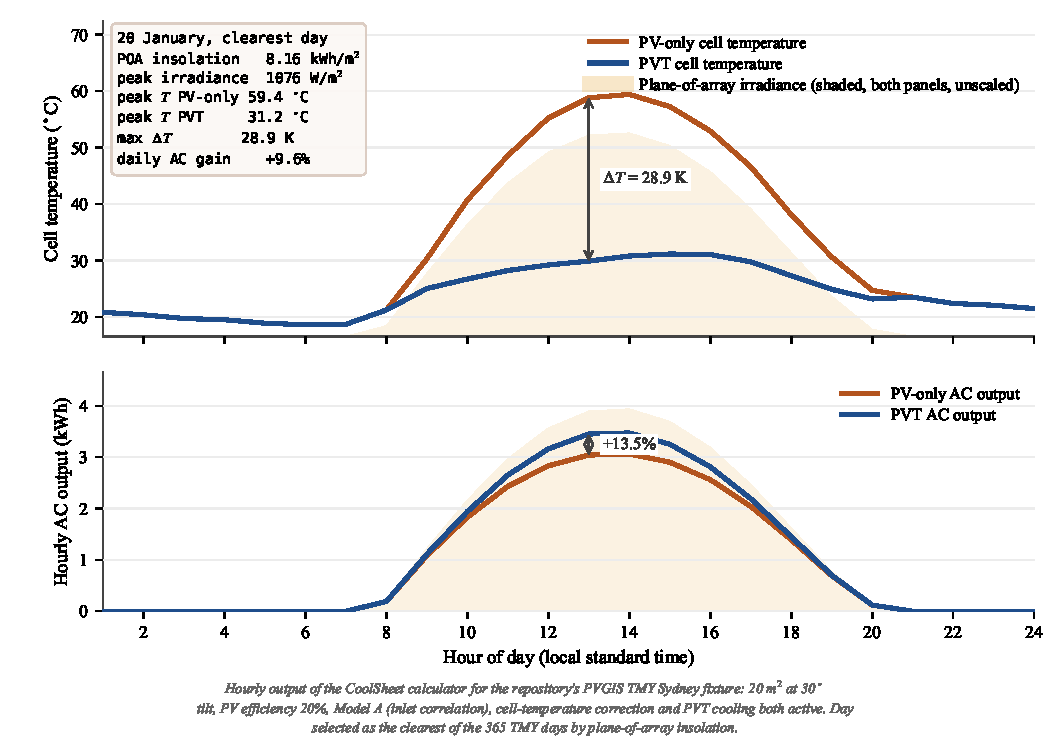
\includegraphics[width=\textwidth]{media/media/fig-IIIF-clearday-cooling-sydney.pdf}
\caption{Modelled cell temperature and alternating-current output with and without PVT cooling, for the clearest day of the Sydney typical meteorological year. Both panels share the hourly time axis and are taken from a single run of the calculator.}
\label{fig:clearday-cooling}
\end{figure}

\subsection[Mains-water temperature results\done]{Mains-water temperature results}\label{sec37}

\begin{spacing}{1.27}
\textbf{Development of the final parameterisation.} Retaining the original $+6^\circ$F offset within a single national Australian fit produced an overall RMSE of 4.590$^\circ$C against the five CER reference profiles. Removing the fixed offset reduced the RMSE to 3.556$^\circ$C, confirming that the original American offset was not generally suitable across the Australian reference climates.\par

\vspace{0.15in}

However, removing the offset only shifted the average level of the predicted profile. It did not account for differences between locations in seasonal amplitude and timing. The final reference-specific fitting approach reduced the overall in-sample RMSE to 0.705$^\circ$C by allowing the offset, amplitude ratio and phase lag to vary between references. Table~\ref{tab:bcaus-rmse-progression} summarises this progression.
\end{spacing}

\begin{table}[htbp]
\centering
\renewcommand{\thetable}{7}
\begin{tabular}{@{}lc@{}}
\toprule
\textbf{Model formulation} & \textbf{Overall RMSE ($^\circ$C)} \\
\midrule
National fit with fixed $+6^\circ$F offset & 4.590 \\
National fit without fixed offset & 3.556 \\
Reference-specific BC-Aus fit & 0.705 \\
\bottomrule
\end{tabular}
\caption{Development of the BC-Aus parameterisation against the CER reference profiles.}
\label{tab:bcaus-rmse-progression}
\end{table}

\begin{spacing}{1.27}
\textbf{Agreement with the CER reference profiles.} The final BC-Aus formulation reproduced the monthly reference profiles with RMSE values ranging from 0.502$^\circ$C for Melbourne to 0.950$^\circ$C for Alice Springs. The maximum monthly absolute deviation among the four runtime references was 1.636$^\circ$C. Table~\ref{tab:bcaus-cer-agreement} lists the location-specific error statistics and Figure~\ref{fig:bcaus-cer} shows the corresponding monthly comparison.
\end{spacing}

\begin{figure}[htbp]
\centering
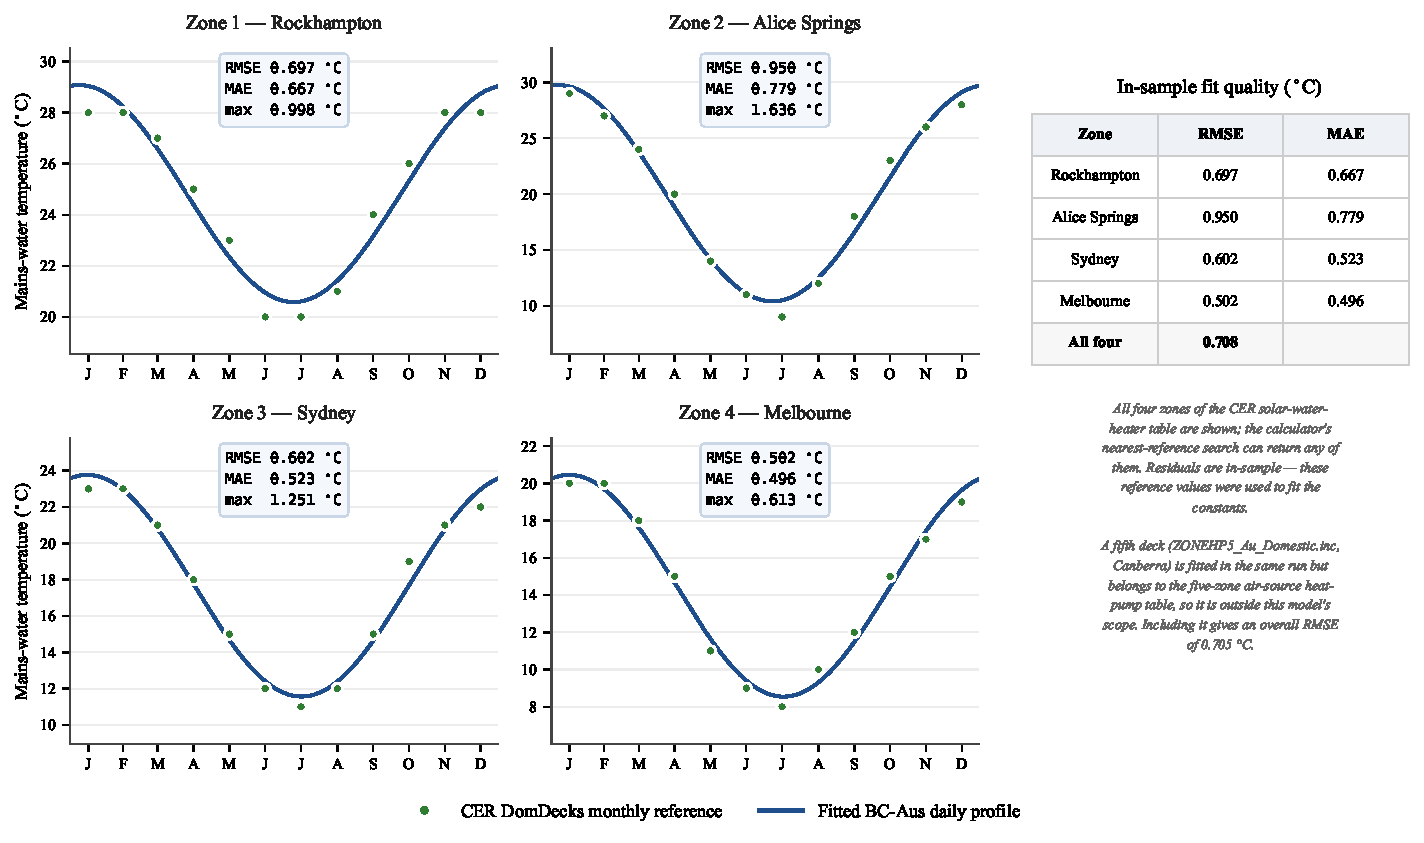
\includegraphics[width=\textwidth]{media/media/fig-IVX-bcaus-4zone-calibration.pdf}
\caption{Fitted BC-Aus daily mains-water profiles against the twelve CER monthly reference values for each of the four solar-water-heater reference locations. Agreement is in-sample: the plotted reference values were used to fit the coefficients.}
\label{fig:bcaus-cer}
\end{figure}

\begin{table}[htbp]
\centering
\renewcommand{\thetable}{8}
\begin{tabular}{@{}lccc@{}}
\toprule
\textbf{Reference location} & \textbf{MAE ($^\circ$C)} & \textbf{RMSE ($^\circ$C)} & \textbf{Maximum absolute error ($^\circ$C)} \\
\midrule
Rockhampton   & 0.667 & 0.697 & 0.998 \\
Alice Springs & 0.779 & 0.950 & 1.636 \\
Sydney        & 0.523 & 0.602 & 1.251 \\
Melbourne     & 0.496 & 0.502 & 0.613 \\
\bottomrule
\end{tabular}
\caption{Agreement between BC-Aus and the CER monthly reference profiles.}
\label{tab:bcaus-cer-agreement}
\end{table}

\begin{spacing}{1.27}
These results demonstrate that the fitted sinusoidal model closely reproduces the available reference profiles. They do not demonstrate equivalent accuracy against actual water temperatures because the CER values were used during model calibration.\par

\vspace{0.15in}

\textbf{Independent physical cross-check.} The final profiles were compared with EnergyPlus undisturbed ground-temperature estimates at 0.5~m and 2.0~m depth. The 0.5~m profiles generally exhibited greater seasonal variation, whereas the deeper profiles showed greater damping. Comparison with both depths provided a useful independent check of seasonal timing and temperature range because the EnergyPlus data were not used during coefficient fitting. EnergyPlus documentation identifies the shallow-ground values as calculated undisturbed temperatures at approximately 0.5~m depth rather than measured mains-water data.
\end{spacing}

\placeholder{[Figure IV.Y to be inserted here -- optional. Comparison of BC-Aus mains-water temperature predictions with EnergyPlus undisturbed ground-temperature estimates at 0.5~m depth, presented as an independent physical proxy rather than measured mains-water temperature. Include only if it fits comfortably within the page limit; requires the actual EnergyPlus comparison data, which has not been supplied yet. The full 2.0~m comparison can remain in the repository validation material or an appendix instead of the main report.]}

\begin{spacing}{1.27}
\textbf{Software verification.} Automated testing confirmed that the correct source identities were associated with the fitted references, the production coefficients could be regenerated deterministically and only the four intended solar-water-heater references could be selected at runtime. Downstream tests also confirmed that colder daily mains-water temperatures increased water-heating demand while warmer temperatures reduced it, without affecting unrelated demand components.\par

\vspace{0.15in}

\textbf{Limitations and interpretation.} No measured Australian mains-water dataset was available for independent validation. The overall RMSE of 0.705$^\circ$C therefore represents agreement with the legacy CER reference profiles used during fitting and must not be interpreted as field prediction accuracy.\par

\vspace{0.15in}

The runtime model also uses the geographically nearest of four reference locations, which may not always be the most climatologically similar reference. Furthermore, the fitted coefficients were derived using the historical weather basis of the CER decks, while runtime calculations use PVGIS TMY statistics for the selected site. EnergyPlus ground temperatures provide an independent physical comparison but remain calculated soil-temperature proxies and do not account for water source, pipe materials, burial geometry, residence time or network operation.\par

\vspace{0.15in}

\textit{The BC-Aus model closely reproduces the available Australian CER cold-water reference profiles and exhibits physically plausible seasonal behaviour relative to independent ground-temperature proxies. Validation against measured mains-water temperatures at independent Australian sites remains necessary before field prediction accuracy can be established.}
\end{spacing}

\subsection{Industry-demand model results}\label{sec38}
% Briefly compare all five: annual demand; demand intensity; load shape; target
% temperatures; seasonality; evidence quality. -- content pending.

\subsection{Principal case study 1}\label{sec39}
% Site/system to be selected. Likely contents: site and system definition; supply profile;
% demand profile; hourly matching; monthly balance; financial results; sensitivity;
% engineering interpretation. -- content pending.

\subsection{Principal case study 2}\label{sec40}
% Choose a contrasting load profile. -- content pending.

\subsection{Cross-industry comparison}\label{sec41}
% Compact comparison of all five industries: thermal solar fraction; electrical solar
% fraction; annual savings; payback; emissions; optimal area; excess energy. -- content
% pending.

\subsection{Sensitivity and sizing analysis}\label{sec42}
% Potential variables: collector area; flow rate; mains-water temperature; energy tariffs;
% boiler efficiency; collector model; climate/location; demand intensity. -- content
% pending.

\subsection{Limitations and uncertainty}\label{sec43}
% TMY rather than measured-year weather; direct use with no storage; simplified demand
% profiles; assumed industry defaults; uncertainty in cooling benefit; field versus
% certified thermal performance; mains model not direct pipe-temperature measurement;
% economics dependent on user assumptions. -- content pending.

\subsection{Engineering significance}\label{sec44}
% Explain what the results mean for: feasibility screening; system sizing; load selection;
% Australian commercial adoption; future development of the tool. -- content pending.

% Likely figures: validation scatter plots; monthly mains profiles; hourly supply--demand
% profiles; monthly matched-energy plots; collector-area sensitivity curves; financial
% sensitivity charts; cross-industry comparison table; uncertainty or validation-status
% matrix.

\clearpage

\section{Conclusions}\label{sec45}
% Target: 1--2 pages. Should not introduce new results or repeat the entire report --
% state the important findings and their significance.

\subsection{Main findings}\label{sec46}
% Directly answer the research question. -- content pending.

\subsection{Contributions}\label{sec47}
% Summarise: integrated hourly tool; mains-water solution; industry-demand models;
% matching and economics; validation and reproducibility. -- content pending.

\subsection{Practical value}\label{sec48}
% State what the calculator can and cannot be used for. -- content pending.

\subsection{Recommendations and future work}\label{sec49}
% Likely items: thermal storage; measured industry data; measured mains-water validation;
% improved PV cooling model; additional industries; uncertainty analysis; calibrated field
% case studies. -- content pending.
\label{sec:bodyend}

\section*{References}\label{sec50}
\phantomsection
\addcontentsline{toc}{section}{References}
% Numbered in order of first appearance; one consistent format; prefer peer-reviewed papers,
% standards and government reports; cite software, datasets and APIs; cite Jianxiong's thesis
% where his prior work is specifically discussed; cite original sources for inherited
% equations rather than relying only on his thesis; check every figure and table source.

\begin{spacing}{1.05}
\footnotesize

\placeholder{NOTE -- entries 1--46 were checked against the published record on 27 July 2026: author lists, titles, volume/article numbers, DOIs and URLs verified. Still to confirm personally: [6] Fu's exact thesis title, and [37] the CoolSheet version and commit identifier once the final case studies are fixed. Delete this note before submission.}

\referenceheading{Industry context and motivation (cited in I.A and I.B)}

\refentry{
\textsuperscript{\refanchor{1}}Australian Renewable Energy Agency, \textit{Renewable Energy for Process Heat Opportunity Study: Final Project Knowledge Sharing Report}, Australian Government, 2022. [Online]. Available: \url{https://arena.gov.au/knowledge-bank/renewable-energy-for-process-heat-opportunity-study-final-report/} (direct report: \url{https://arena.gov.au/assets/2022/03/renewable-energy-for-process-heat-opportunity-study-final-report.pdf}). \textit{[Accessed: 26 July 2026]}
}

\refentry{
\textsuperscript{\refanchor{2}}Australian PV Institute and UNSW Sydney, ``SunSPOT solar and battery calculator.'' [Online]. Available: \url{https://www.sunspot.org.au/} (tool information: \url{https://www.sunspot.org.au/about-sunspot-solar-tool}). \textit{[Accessed: 26 July 2026]}
}

\refentry{
\textsuperscript{\refanchor{3}}National Renewable Energy Laboratory, ``PVWatts Calculator.'' [Online]. Available: \url{https://pvwatts.nrel.gov/} (Version 8 information: \url{https://pvwatts.nrel.gov/version_8.php}). \textit{[Accessed: 26 July 2026] -- source text said ``National Laboratory of the Rockies,'' corrected to National Renewable Energy Laboratory (NREL); source text also gave the URL as pvwatts.nlr.gov, which appears to be a typo for pvwatts.nrel.gov.}
}

\refentry{
\textsuperscript{\refanchor{4}}International Energy Agency Solar Heating and Cooling Programme, ``PVT systems: Heat or electricity from solar -- Why only one when you can have both?,'' \textit{SHC Solar Update}, Task 60, July 2021. [Online]. Available: \url{https://task60.iea-shc.org/Data/Sites/1/publications/2021-07-Task60-PVT-Systems.pdf}.
}

\refentry{
\textsuperscript{\refanchor{5}}International Energy Agency Solar Heating and Cooling Programme, \textit{Performance Assessment of Example PVT Systems}, Task 60, 2020. [Online]. Available: \url{https://www.iea-shc.org/Data/Sites/1/publications/IEA-SHC-Task60-2020-System-Evaluation.pdf}.
}

\referenceheading{Prior collaborative work (cited in I.E)}

\refentry{
\textsuperscript{\refanchor{6}}Fu, J., \textit{The Development of Web-Based Calculator for Hourly Outputs of Photovoltaic-Thermal Systems}, Master's Thesis, UNSW Sydney, 2026.
}

\referenceheading{Photovoltaic-thermal systems (cited in II.A)}

\refentry{
\textsuperscript{\refanchor{7}}International Electrotechnical Commission, \textit{IEC 60891:2021 -- Photovoltaic Devices: Procedures for Temperature and Irradiance Corrections to Measured I--V Characteristics}, Geneva, 2021, with Corrigendum 1, 2024. [Online]. Available: \url{https://webstore.iec.ch/en/publication/61766} (Corrigendum: \url{https://webstore.iec.ch/en/publication/88173}). \textit{[Accessed: 26 July 2026]}
}

\refentry{
\textsuperscript{\refanchor{8}}Advanced Manufacturing Growth Centre, ``Manufacture of energy efficient PVT CoolSheet system,'' 2021. [Online]. Available: \url{https://www.amgc.org.au/project/manufacture-of-energy-efficient-pvt-coolsheet-system/}. \textit{[Accessed: 26 July 2026]}
}

\referenceheading{Environmental effects on PVT performance (cited in II.B)}

\refentry{
\textsuperscript{\refanchor{9}}Yildirim, M. A., Cebula, A., and Sułowicz, M., ``A cooling design for photovoltaic panels -- Water-based PV/T system,'' \textit{Energy}, Vol. 256, Art. 124654, 2022. DOI: \url{https://doi.org/10.1016/j.energy.2022.124654}.
}

\refentry{
\textsuperscript{\refanchor{10}}Basuhaib, A., Selvaraj, J., Hasanuzzaman, M., Anjum, T., and Kumar, L., ``Experimental investigation the effect of different operating parameters and optimized the water-based PVT system for domestic applications,'' \textit{Solar Energy}, Vol. 268, Art. 112278, 2024. DOI: \url{https://doi.org/10.1016/j.solener.2023.112278}.
}

\refentry{
\textsuperscript{\refanchor{11}}Hassanian, R., Yeganeh, N., and Riedel, M., ``Wind velocity and forced heat transfer model for photovoltaic module,'' \textit{Fluids}, Vol. 9, No. 1, Art. 17, 2024. DOI: \url{https://doi.org/10.3390/fluids9010017}.
}

\refentry{
\textsuperscript{\refanchor{12}}Tripty, T. A., and Nasrin, R., ``Efficiency upgrading of solar PVT finned hybrid system in Bangladesh: Flow rate and temperature influences,'' \textit{Heliyon}, Vol. 10, No. 7, Art. e28323, 2024. DOI: \url{https://doi.org/10.1016/j.heliyon.2024.e28323}.
}

\referenceheading{Hourly weather and solar-resource modelling (cited in II.C)}

\refentry{
\textsuperscript{\refanchor{13}}Bureau of Meteorology, ``Himawari-8/9 surface global solar irradiance,'' Australian Government, updated 2025. [Online]. Available: \url{https://www.bom.gov.au/climate/how/newproducts/himawari-irradiance.shtml}. \textit{[Accessed: 26 July 2026]}
}

\refentry{
\textsuperscript{\refanchor{14}}European Commission, Joint Research Centre, ``PVGIS typical meteorological year generator.'' [Online]. Available: \url{https://joint-research-centre.ec.europa.eu/photovoltaic-geographical-information-system-pvgis/using-pvgis-5/pvgis-5-tools/pvgis-typical-meteorological-year-tmy-generator_en}. \textit{[Accessed: 26 July 2026]}
}

\refentry{
\textsuperscript{\refanchor{15}}Kulesza, K., Martinez, A., and Taylor, N., ``Assessment of Typical Meteorological Year Data in Photovoltaic Geographical Information System 5.2, Based on Reanalysis and Ground Station Data from 147 European Weather Stations,'' \textit{Atmosphere}, Vol. 14, No. 12, Art. 1803, 2023. DOI: \url{https://doi.org/10.3390/atmos14121803}.
}

\refentry{
\textsuperscript{\refanchor{16}}Bureau of Meteorology, ``Solar and terrestrial radiation glossary,'' Australian Government. [Online]. Available: \url{https://www.bom.gov.au/climate/austmaps/solar-radiation-glossary.shtml}. \textit{[Accessed: 26 July 2026]}
}

\refentry{
\textsuperscript{\refanchor{17}}European Commission, Joint Research Centre, ``PVGIS hourly radiation.'' [Online]. Available: \url{https://joint-research-centre.ec.europa.eu/photovoltaic-geographical-information-system-pvgis/using-pvgis-5/pvgis-5-tools/hourly-radiation_en}. \textit{[Accessed: 26 July 2026]}
}

\refentry{
\textsuperscript{\refanchor{18}}pvlib Python Development Team, ``Irradiance transposition models,'' pvlib Python Documentation. [Online]. Available: \url{https://pvlib-python.readthedocs.io/en/stable/reference/irradiance/transposition.html}. \textit{[Accessed: 26 July 2026]}
}

\referenceheading{PVT thermal and electrical models (cited in II.D)}

\refentry{
\textsuperscript{\refanchor{19}}International Organization for Standardization, \textit{ISO 9806:2025 -- Solar Thermal Collectors: Test Methods}, 3rd ed., Geneva, 2025. [Online]. Available: \url{https://www.iso.org/standard/78801.html}.
}

\refentry{
\textsuperscript{\refanchor{20}}International Energy Agency Solar Heating and Cooling Programme, \textit{Status Quo of PVT Characterization}, Task 60, Report B1, 2020. [Online]. Available: \url{https://www.iea-shc.org/Data/Sites/1/publications/IEA-SHC-Task60-B1-Status-Quo-Report-PVT-Characterization.pdf}.
}

\refentry{
\textsuperscript{\refanchor{21}}International Energy Agency Solar Heating and Cooling Programme, \textit{Numerical Simulation Tools for PVT Collectors and Systems}, Task 60, 2020. [Online]. Available: \url{https://task60.iea-shc.org/Data/Sites/1/publications/IEA-SHC-Task60-Numerical-Ssimulations-for-PVT.pdf}.
}

\refentry{
\textsuperscript{\refanchor{22}}pvlib Python Development Team, ``PVWatts DC power model,'' pvlib Python Documentation. [Online]. Available: \url{https://pvlib-python.readthedocs.io/en/stable/reference/generated/pvlib.pvsystem.pvwatts_dc.html}. \textit{[Accessed: 26 July 2026]}
}

\refentry{
\textsuperscript{\refanchor{23}}pvlib Python Development Team, ``PV module and cell-temperature models,'' pvlib Python Documentation. [Online]. Available: \url{https://pvlib-python.readthedocs.io/en/stable/reference/pv_modeling/temperature.html}. \textit{[Accessed: 26 July 2026]}
}

\referenceheading{Mains-water temperature (cited in II.E and III.F)}

\refentry{
\textsuperscript{\refanchor{24}}Bors, J., O'Brien, K. R., Kenway, S. J., and Lant, P. A., ``Regional-scale variability of cold water temperature: Implications for household water-related energy demand,'' \textit{Resources, Conservation and Recycling}, Vol. 124, 2017, pp. 107--115. DOI: \url{https://doi.org/10.1016/j.resconrec.2017.05.001}.
}

\refentry{
\textsuperscript{\refanchor{25}}Ren, Z., Chan, W. Y., and Chen, D., \textit{Addition of a Hot-Water Module to AccuRate}, report for the Australian Government Department of the Environment, Water, Heritage and the Arts, 2009. [Online]. Available: \url{https://www.homeenergyrating.gov.au/resources/addition-hot-water-module-accurate}. \textit{[Accessed: 26 July 2026]}
}

\refentry{
\textsuperscript{\refanchor{26}}Burch, J., and Christensen, C., ``Towards Development of an Algorithm for Mains Water Temperature,'' \textit{Proceedings of the American Solar Energy Society Annual Conference}, Cleveland, OH, 2007. [Online]. Available: \url{https://www.osti.gov/biblio/981988}.
}

\refentry{
\textsuperscript{\refanchor{27}}Hendron, R., and Engebrecht, C., \textit{Building America House Simulation Protocols}, NREL/TP-550-49426, 2010. [Online]. Available: \url{https://www.osti.gov/biblio/989422}. DOI: \url{https://doi.org/10.2172/989422}.
}

\referenceheading{Industrial energy-demand modelling (cited in II.F)}

\refentry{
\textsuperscript{\refanchor{28}}Dairy Australia, ``Manufacturing sustainability resources.'' [Online]. Available: \url{https://www.dairyaustralia.com.au/manufacturing-support/manufacturing-sustainability/resources}. \textit{[Accessed: 26 July 2026]}
}

\referenceheading{Techno-economic evaluation (cited in II.G)}

\refentry{
\textsuperscript{\refanchor{29}}National Renewable Energy Laboratory, ``System Advisor Model.'' [Online]. Available: \url{https://sam.nrel.gov/} (solar-water-heating model: \url{https://sam.nrel.gov/solar-water-heating.html}; residential and commercial financial models: \url{https://sam.nrel.gov/financial-models/residential-and-commercial.html}). \textit{[Accessed: 26 July 2026] -- source text said ``National Laboratory of the Rockies,'' corrected to National Renewable Energy Laboratory (NREL).}
}

\refentry{
\textsuperscript{\refanchor{30}}He, Y., Song, J., Guo, S., Zhou, J., and Markides, C. N., ``A techno-economic-environmental comparison of residential solar energy systems employing an up-to-date market analysis,'' \textit{Energy Conversion and Management}, Vol. 345, Art. 120357, 2025. DOI: \url{https://doi.org/10.1016/j.enconman.2025.120357} (author manuscript: \url{https://research.chalmers.se/publication/547975/file/547975_Fulltext.pdf}).
}

\refentry{
\textsuperscript{\refanchor{31}}Department of Climate Change, Energy, the Environment and Water, \textit{National Greenhouse Accounts Factors 2025}, Australian Government, 2025. [Online]. Available: \url{https://www.dcceew.gov.au/climate-change/publications/national-greenhouse-accounts-factors-2025} (direct report: \url{https://www.dcceew.gov.au/sites/default/files/documents/national-greenhouse-account-factors-2025.pdf}).
}

\referenceheading{Existing simulation and web tools (cited in II.H)}

\refentry{
\textsuperscript{\refanchor{32}}Thermal Energy System Specialists, ``TRNSYS: Transient System Simulation Tool.'' [Online]. Available: \url{https://www.trnsys.com/} (features: \url{https://www.trnsys.com/features/}; component libraries: \url{https://www.trnsys.com/features/libraries.php.html}; TESS PVT components: \url{https://www.trnsys.com/tess-libraries/}). \textit{[Accessed: 26 July 2026]}
}

\refentry{
\textsuperscript{\refanchor{33}}Vela Solaris, ``Polysun energy-modelling software.'' [Online]. Available: \url{https://www.velasolaris.com/en/} (PVT collector modelling: \url{https://www.velasolaris.com/en/handbuch/polysun-designer/producers/solar-thermal-collectors/pvt-collectors/}; simulation analysis: \url{https://www.velasolaris.com/en/handbuch/polysun-designer/results-and-analysis/simulation-analysis/}). \textit{[Accessed: 26 July 2026]}
}

\referenceheading{Software and data sources (cited in III.A, III.B and III.C)}

\refentry{
\textsuperscript{\refanchor{34}}Nominatim, ``Search API,'' \textit{Nominatim Manual}. [Online]. Available: \url{https://nominatim.org/release-docs/latest/api/Search/}. \textit{[Accessed: 27 July 2026]}
}

\refentry{
\textsuperscript{\refanchor{35}}European Commission, Joint Research Centre, ``Photovoltaic Geographical Information System (PVGIS),'' Version 5.3. [Online]. Available: \url{https://re.jrc.ec.europa.eu/pvg_tools/en/}. \textit{[Accessed: 27 July 2026]}
}

\refentry{
\textsuperscript{\refanchor{36}}Holmgren, W. F., Hansen, C. W., and Mikofski, M. A., ``pvlib python: A Python Package for Modeling Solar Energy Systems,'' \textit{Journal of Open Source Software}, Vol. 3, No. 29, Art. 884, 2018. DOI: \url{https://doi.org/10.21105/joss.00884}.
}

\refentry{
\textsuperscript{\refanchor{37}}CoolSheet PVT Calculator, ``Source code, validation material and model implementation.'' [Online]. Available: \url{https://github.com/coolsheet-pvt/coolsheet-pvt.github.io}. \textit{-- add the version and commit identifier used for the final case studies before submission.}
}

\refentry{
\textsuperscript{\refanchor{38}}European Commission, Joint Research Centre, ``Typical Meteorological Year,'' JRC Data Catalogue. [Online]. Available: \url{https://re.jrc.ec.europa.eu/pvg_tools/en/}. \textit{[Accessed: 26 July 2026]}
}

\referenceheading{Solar geometry and irradiance transposition (cited in III.D)}

\refentry{
\textsuperscript{\refanchor{39}}Cooper, P. I., ``The absorption of radiation in solar stills,'' \textit{Solar Energy}, Vol. 12, No. 3, pp. 333--346, 1969. DOI: \url{https://doi.org/10.1016/0038-092X(69)90047-4}.
}

\refentry{
\textsuperscript{\refanchor{40}}Duffie, J. A., and Beckman, W. A., \textit{Solar Engineering of Thermal Processes}, 4th ed., Hoboken, NJ: John Wiley \& Sons, 2013. DOI: \url{https://doi.org/10.1002/9781118671603}.
}

\refentry{
\textsuperscript{\refanchor{41}}Liu, B. Y. H., and Jordan, R. C., ``The long-term average performance of flat-plate solar-energy collectors,'' \textit{Solar Energy}, Vol. 7, No. 2, pp. 53--74, 1963. DOI: \url{https://doi.org/10.1016/0038-092X(63)90006-9}.
}

\referenceheading{PVT supply model (cited in III.E)}

\refentry{
\textsuperscript{\refanchor{42}}International Organization for Standardization, \textit{ISO 9806:2017 -- Solar Energy: Solar Thermal Collectors -- Test Methods}, Geneva, 2017. [Online]. Available: \url{https://www.iso.org/standard/67978.html}. \textit{The implementation uses the 2017 formulation on which the frozen model was based.}
}

\refentry{
\textsuperscript{\refanchor{43}}Dobos, A. P., \textit{PVWatts Version 5 Manual}, NREL/TP-6A20-62641, National Renewable Energy Laboratory, Golden, CO, 2014. [Online]. Available: \url{https://www.nrel.gov/docs/fy14osti/62641.pdf}. DOI: \url{https://doi.org/10.2172/1158421}.
}

\referenceheading{Software implementation and deployment (cited in III.K and the appendices)}

\refentry{
\textsuperscript{\refanchor{44}}Ram\'irez, S., ``FastAPI documentation.'' [Online]. Available: \url{https://fastapi.tiangolo.com/}. \textit{[Accessed: 27 July 2026]}
}

\refentry{
\textsuperscript{\refanchor{45}}GitHub, Inc., ``What is GitHub Pages?'' GitHub Docs. [Online]. Available: \url{https://docs.github.com/en/pages/getting-started-with-github-pages/what-is-github-pages}. \textit{[Accessed: 27 July 2026]}
}

\referenceheading{Economic evaluation methods (cited in III.I)}

\refentry{
\textsuperscript{\refanchor{46}}Short, W., Packey, D. J., and Holt, T., \textit{A Manual for the Economic Evaluation of Energy Efficiency and Renewable Energy Technologies}, NREL/TP-462-5173, National Renewable Energy Laboratory, Golden, CO, 1995. [Online]. Available: \url{https://docs.nrel.gov/docs/legosti/old/5173.pdf}. \textit{The SAM documentation identifies this handbook as the basis for its principal financial metrics.}
}

\referenceheading{Dairy energy benchmarks (cited in III.G.1)}

\refentry{
\textsuperscript{\refanchor{47}}Clack, S., ``Saving energy on dairy farms,'' \textit{Energy Smart Farming}, Agriculture Victoria, 16 February 2024. [Online]. Available: \url{https://extensionaus.com.au/energysmartfarming/saving-energy-on-dairy-farms/}. \textit{[Accessed: 27 July 2026]}
}

\refentry{
\textsuperscript{\refanchor{48}}Subtropical Dairy, \textit{Dairy Shed Energy Use Check}, Dairy Australia. [Online]. Available: \url{https://northernaustraliandairyhub.com.au/wp-content/uploads/2020/10/Dairy-Shed-Energy-Use-Check.pdf}. \textit{[Accessed: 27 July 2026]}
}

\end{spacing}

\clearpage
\mbox{}
\thispagestyle{plain}
\clearpage

\section*{Appendices}\label{sec51}
\phantomsection
\addcontentsline{toc}{section}{Appendices}
% WORKING NOTE -- appends the page-budget table to the end of the Contents listing,
% directly under the Appendices entry. DELETE BEFORE SUBMISSION (see \pagebudgettable).
\addtocontents{toc}{\protect\pagebudgettable}
% Keep supporting detail out of the main engineering story. Possible appendices: full model
% equations; industry-input tables; fitted mains-water coefficients; validation test
% inventory; additional case-study results; sensitivity tables; user-interface screenshots;
% code and repository information; sample hourly CSV output; contribution statement.

\referenceheading{Appendix A --- Calculator input register, model coefficients and solver configuration}

\begin{spacing}{1.27}
Tables~\ref{tab:reg-site}--\ref{tab:reg-coeffs} record every parameter the calculator reads, with its interface label, the identifier used in the source, units, the value shipped with the application and the accepted range or validation rule. \textit{User} denotes a value entered directly, \textit{derived} a value the software computes from other inputs, and \textit{optional} a toggle or override that is inactive unless selected. Ranges given as ``clamped'' are silently constrained to the stated interval rather than rejected; ranges given as limits are rejected with a message. Blank or non-numeric entries fall back to the shipped default, except where a fallback is stated separately.\par
\end{spacing}

\vspace{0.1in}

\begin{table}[htbp]
\centering
\footnotesize
\setlength{\tabcolsep}{4pt}
\begin{tabular}{@{}>{\raggedright\arraybackslash}p{1.30in}>{\raggedright\arraybackslash}p{1.55in}>{\raggedright\arraybackslash}p{0.60in}>{\raggedright\arraybackslash}p{0.50in}>{\raggedright\arraybackslash}p{1.25in}>{\raggedright\arraybackslash}p{0.48in}@{}}
\toprule
\textbf{Interface label} & \textbf{Identifier} & \textbf{Unit} & \textbf{Default} & \textbf{Range or rule} & \textbf{Type} \\
\midrule
Address & \path{addressInput} & -- & (blank) & geocoded; warning if outside Australia & user \\
Collector / PV area & \path{area} & m$^2$ & 250 & $>0$ & user \\
Panel tilt & \path{tiltAngle} & $^\circ$ & 30 & 0--90 & user \\
Panel direction & \path{azimuthAngle} & $^\circ$ & 0 & $-180$ to $+180$; $0^\circ$ = north & user \\
Ground reflectivity & \path{albedo} & -- & 0.2 & 0--1 & user \\
Water flow rate & \path{flowRate} & L\,s$^{-1}$m$^{-2}$ & 0.02 & $>0$ & user \\
Panel efficiency & \path{etaPvPercent} & \% & 20 & 0--100 & user \\
PV temperature loss & \path{pvTempCoeff} & \%\,$^\circ$C$^{-1}$ & $-0.40$ & finite; $-0.40$ if blank & user \\
NOCT panel temperature & \path{pvNoct} & $^\circ$C & 45 & 20--80 & user \\
Non-inverter system losses & \path{pvSystemLossPct} & \% of DC & 14 & clamped 0--99 & user \\
Inverter efficiency & \path{pvInverterEfficiencyPct} & \% & 96 & clamped 1--100 & user \\
Module temperature correction & \path{pvTempCorrEnable} & -- & on & forced on outside diagnostic mode & optional \\
PVT cooling sensitivity & \path{pvtCoolingSensitivityEnable} & -- & on & forced on outside diagnostic mode & optional \\
Thermal model & \path{thermalModel} & -- & A & A or B & user \\
Custom monthly mains temperatures & \path{mainsCustomEnable} & -- & off & on or off & optional \\
Monthly mains temperature & \path{mainsM0}--\path{mainsM11} & $^\circ$C & from model & blank months use the modelled daily value & optional \\
Set all months to & \path{mainsQuickSet} & $^\circ$C & (blank) & finite; enables custom mode & optional \\
Diagnostic mode & \path{chkHideMains} & -- & off & on or off & optional \\
\bottomrule
\end{tabular}
\renewcommand{\thetable}{9}
\caption{Site, PVT system and mains-override input register.}
\label{tab:reg-site}
\end{table}

% Set as a longtable because the register runs past a single page. \thetable is
% overridden inside a group so the fixed display number cannot leak into later tables.
\begingroup
\renewcommand{\thetable}{10}
\footnotesize
\setlength{\tabcolsep}{4pt}
\begin{longtable}{@{}>{\raggedright\arraybackslash}p{1.28in}>{\raggedright\arraybackslash}p{1.52in}>{\raggedright\arraybackslash}p{0.70in}>{\raggedright\arraybackslash}p{0.58in}>{\raggedright\arraybackslash}p{1.05in}>{\raggedright\arraybackslash}p{0.48in}@{}}
\caption{Industry-demand input register. Process-selection checkboxes are additionally provided for each industry, all selected by default.}
\label{tab:reg-industry}\\
\toprule
\textbf{Interface label} & \textbf{Identifier} & \textbf{Unit} & \textbf{Default} & \textbf{Range or rule} & \textbf{Type} \\
\midrule
\endfirsthead
\toprule
\textbf{Interface label} & \textbf{Identifier} & \textbf{Unit} & \textbf{Default} & \textbf{Range or rule} & \textbf{Type} \\
\midrule
\endhead
\bottomrule
\endlastfoot
\multicolumn{6}{@{}l}{\textit{All industries}} \\
Industry & \path{industrySelect} & -- & none & one of five models & user \\
Operating profile & \path{profileType} & -- & 24/7 & continuous or Mon--Fri & user \\
Throughput per year & \path{throughputInput} & L\,yr$^{-1}$ & 5{,}000{,}000 & $>0$; dairy and brewery only & user \\
\addlinespace
\multicolumn{6}{@{}l}{\textit{Dairy farm}} \\
Electricity intensity & \path{dairyElectricKWhPerKL} & kWh\,kL$^{-1}$ & 51.7 & $\geq 0$ & user \\
Fatty-film rinse water & \path{dairyFattyWater} & L\,L$^{-1}$ & 0.30 & $\geq 0$ & user \\
CIP preheat water & \path{dairyCipWater} & L\,L$^{-1}$ & 0.57 & $\geq 0$ & user \\
Boiler preheat water & \path{dairyBoilerWater} & L\,L$^{-1}$ & 0.50 & $\geq 0$ & user \\
Preheat target & \path{dairyTargetTemp} & $^\circ$C & 35 & clamped 15--95; shared by all three processes & user \\
\addlinespace
\multicolumn{6}{@{}l}{\textit{Brewery}} \\
Electricity intensity & \path{breweryElectricKWhPerHL} & kWh\,hL$^{-1}$ & 11.5 & $\geq 0$ & user \\
CIP pre-rinse water & \path{breweryCipWater} & L\,L$^{-1}$ & 0.80 & $\geq 0$ & user \\
Bottle/keg rinse water & \path{breweryRinseWater} & L\,L$^{-1}$ & 0.45 & $\geq 0$ & user \\
Boiler preheat water & \path{breweryBoilerWater} & L\,L$^{-1}$ & 0.60 & $\geq 0$ & user \\
CIP/boiler target & \path{breweryCipTarget} & $^\circ$C & 45 & clamped 15--95 & user \\
Bottle/keg rinse target & \path{breweryRinseTarget} & $^\circ$C & 40 & clamped 15--95 & user \\
\addlinespace
\multicolumn{6}{@{}l}{\textit{Hotel}} \\
Total available rooms & \path{hotelRoomsInput} & -- & 147 & $>0$ & user \\
Occupancy rate & \path{hotelOccupancyInput} & \% & 73.4 & 0--100 & user \\
Occupied room-nights & (derived) & yr$^{-1}$ & 39{,}383 & rooms $\times\,365\times$ occupancy & derived \\
Domestic hot water & \path{hotelDhwKWh} & kWh\,unit$^{-1}$ & 4.5 & $\geq 0$ & user \\
Kitchen/dishwashing & \path{hotelKitchenKWh} & kWh\,unit$^{-1}$ & 1.6 & $\geq 0$ & user \\
Laundry & \path{hotelLaundryKWh} & kWh\,unit$^{-1}$ & 1.2 & $\geq 0$ & user \\
Pool heating & \path{hotelPoolKWh} & kWh\,unit$^{-1}$ & 4.2 & $\geq 0$ & user \\
Whole-site electricity & \path{hotelElectricKWh} & kWh\,unit$^{-1}$ & 15 & $\geq 0$ & user \\
Metered annual fuel & \path{hotelMeasuredAnnualFuelGj} & GJ & (blank) & $\geq 0$ & optional \\
Apply meter calibration & \path{hotelApplyMeterCalibration} & -- & off & on or off & optional \\
Monthly metered fuel & \path{hotelMeterJanFuelGj}\,\ldots & GJ & (blank) & twelve fields, $\geq 0$ & optional \\
\addlinespace
\multicolumn{6}{@{}l}{\textit{Aquatic centre}} \\
Indoor pool area & \path{aquaticIndoorArea} & m$^2$ & 350 & $\geq 0$ & user \\
Outdoor pool area & \path{aquaticOutdoorArea} & m$^2$ & 250 & $\geq 0$ & user \\
Kids pool area & \path{aquaticKidsArea} & m$^2$ & 90 & $\geq 0$ & user \\
Sauna area & \path{aquaticSaunaArea} & m$^2$ & 25 & $\geq 0$ & user \\
Pool cover off-hours & \path{aquaticPoolCover} & -- & on & on or off & optional \\
Electricity assumption & \path{aquaticElectricKWhPerM2} & kWh\,m$^{-2}$yr$^{-1}$ & 250 & $\geq 0$ & user \\
Evaporation multiplier & \path{aquaticEvaporationScale} & -- & 1 & clamped 0--3 & user \\
Makeup-water multiplier & \path{aquaticMakeupScale} & -- & 1 & clamped 0--3 & user \\
\addlinespace
\multicolumn{6}{@{}l}{\textit{Commercial laundry}} \\
Laundry processed & \path{laundryKgPerDay} & kg\,day$^{-1}$ & 1{,}500 & $\geq 0$ & user \\
Operating days per week & \path{laundryOperatingDaysPerWeek} & -- & 6 & clamped 0--7 & user \\
Wash hot-water target & \path{laundryWashTempC} & $^\circ$C & 60 & clamped 20--95 & user \\
Total wash water & \path{laundryWaterUseLPerKg} & L\,kg$^{-1}$ & 10 & $\geq 0$ & user \\
Water-use scenario & \path{laundryWaterScenario} & L\,kg$^{-1}$ & custom & presets 10, 12, 15, 17, 22 & optional \\
Hot-water fraction & \path{laundryHotWaterFraction} & -- & 0.65 & clamped 0--1 & user \\
Warm-rinse fraction & \path{laundryWarmRinseFraction} & -- & 0.20 & clamped 0--1 & user \\
Warm-rinse target & \path{laundryWarmRinseTempC} & $^\circ$C & 35 & clamped 15--60 & user \\
System loss fraction & \path{laundrySystemLossFraction} & -- & 0 & clamped 0--1 & user \\
\end{longtable}
\endgroup

\begin{table}[htbp]
\centering
\footnotesize
\setlength{\tabcolsep}{4pt}
\begin{tabular}{@{}>{\raggedright\arraybackslash}p{1.30in}>{\raggedright\arraybackslash}p{1.55in}>{\raggedright\arraybackslash}p{0.72in}>{\raggedright\arraybackslash}p{0.42in}>{\raggedright\arraybackslash}p{1.18in}>{\raggedright\arraybackslash}p{0.50in}@{}}
\toprule
\textbf{Interface label} & \textbf{Identifier} & \textbf{Unit} & \textbf{Default} & \textbf{Range or rule} & \textbf{Type} \\
\midrule
Electricity bought from grid & \path{electricityPrice} & AUD\,kWh$^{-1}$ & 0.27 & $\geq 0$ & user \\
Electricity exported to grid & \path{feedInTariffInput} & AUD\,kWh$^{-1}$ & 0.06 & $\geq 0$ & user \\
Natural gas price & \path{gasPriceInput} & AUD\,MJ$^{-1}$ & 0.020 & $\geq 0$ & user \\
Existing boiler efficiency & \path{boilerEffInput} & -- & 0.85 & clamped 0.5--1 & user \\
Region for emissions estimate & \path{gridEmissionFactor} & kg\,CO$_2$-e per kWh & 0.62 & 0.20--0.78 by region & user \\
Fill installed cost from \$/W & \path{autoCapexFromWatts} & -- & \textbf{on} & on or off & optional \\
PV installed cost & \path{pvInstalledCostPerW} & AUD\,W$^{-1}$ & 1.20 & $\geq 0$ & user \\
Thermal / PVT installed cost & \path{thermalInstalledCostPerW} & AUD\,W$^{-1}$ & 1.50 & $\geq 0$ & user \\
Installed cost & \path{capexInput} & AUD\,m$^{-2}$ & 800 & $\geq 0$; overwritten with 540 while auto-fill is on & user or derived \\
Calculated CAPEX & \path{calculatedCapexPerM2} & AUD\,m$^{-2}$ & 540 & read-only & derived \\
Installed cost conversion & \path{installedCostPerFt2} & AUD\,ft$^{-2}$ & 50.17 & read-only & derived \\
Annual operating cost & \path{opexRateInput} & \% of $C_0$ & 1.5 & 0--20 & user \\
System lifetime & \path{systemLifeInput} & yr & 25 & 1--50, floored to integer & user \\
Discount rate & \path{discountRateInput} & \% & 6 & 0--30 & user \\
Target heat coverage & \path{designExplorerTargetInput} & \% & from result & clamped 1--99 & user \\
\bottomrule
\end{tabular}
\renewcommand{\thetable}{11}
\caption{Economics, emissions, finance and sizing input register.}
\label{tab:reg-econ}
\end{table}

\begin{table}[htbp]
\centering
\footnotesize
\setlength{\tabcolsep}{4pt}
\begin{tabular}{@{}>{\raggedright\arraybackslash}p{2.05in}>{\raggedright\arraybackslash}p{0.72in}>{\raggedright\arraybackslash}p{1.32in}>{\raggedright\arraybackslash}p{1.55in}@{}}
\toprule
\textbf{Quantity} & \textbf{Symbol} & \textbf{Stored value} & \textbf{Unit} \\
\midrule
\multicolumn{4}{@{}l}{\textit{Model A --- inlet-temperature correlation}} \\
Zero-loss coefficient & $a_{0,\mathrm{A}}$ & 0.279952866 & -- \\
Inlet-temperature loss coefficient & $a_{1,\mathrm{A}}$ & $-10.52839866$ & W\,m$^{-2}$K$^{-1}$ \\
Wind-speed coefficient & $a_{2,\mathrm{A}}$ & $-0.008135537$ & s\,m$^{-1}$ \\
\addlinespace
\multicolumn{4}{@{}l}{\textit{Model B --- ISO 9806 formulation}} \\
Zero-loss efficiency & $\eta_0$ & 0.762 & -- \\
Linear heat-loss coefficient & $a_1$ & 3.93 & W\,m$^{-2}$K$^{-1}$ \\
Quadratic heat-loss coefficient & $a_2$ & 0.0095 & W\,m$^{-2}$K$^{-2}$ \\
Wind$\times$temperature loss & $a_3$ & 0 & J\,m$^{-3}$K$^{-1}$ \\
Sky-temperature coefficient & $a_4$ & 0 & -- \\
Wind$\times$irradiance coefficient & $a_6$ & 0 & s\,m$^{-1}$ \\
Fourth-order loss coefficient & $a_8$ & 0 & W\,m$^{-2}$K$^{-4}$ \\
\addlinespace
\multicolumn{4}{@{}l}{\textit{Newton--Raphson solver (Model B only)}} \\
Initial outlet estimate & $T_{\mathrm{out}}^{(0)}$ & 40 & $^\circ$C \\
Iteration cap & -- & 5 & interface range 1--10 \\
Convergence tolerance on $\Delta T_{\mathrm{out}}$ & -- & $1\times10^{-4}$ & $^\circ$C \\
Minimum Jacobian magnitude & -- & $1\times10^{-12}$ & W\,K$^{-1}$ \\
\addlinespace
\multicolumn{4}{@{}l}{\textit{Fixed physical constants}} \\
Water specific heat & $c_p$ & 4184 & J\,kg$^{-1}$K$^{-1}$ \\
Water specific heat (demand and outlet terms) & $c_p$ & 4.184 & kJ\,kg$^{-1}$K$^{-1}$ \\
Water density (implicit, not a named constant) & $\rho_{\mathrm{w}}$ & 1 & kg\,L$^{-1}$ \\
Stefan--Boltzmann constant & $\sigma$ & $5.67\times10^{-8}$ & W\,m$^{-2}$K$^{-4}$ \\
Sky long-wave irradiance & $E_{\mathrm{L}}$ & $5.31\times10^{-13}\,T_{\mathrm{a,K}}^{6}$ & W\,m$^{-2}$ \\
Standard test cell temperature & -- & 25 & $^\circ$C \\
NOCT reference irradiance and ambient & -- & 800 and 20 & W\,m$^{-2}$ and $^\circ$C \\
Latent heat of evaporation (aquatic) & -- & 0.680 & kWh\,kg$^{-1}$ \\
Natural-gas emissions factor & $EF_{\mathrm{gas}}$ & 51.53 & kg\,CO$_2$-e\,GJ$^{-1}$ \\
Energy unit conversion & -- & $1000/3.6$ & kWh\,GJ$^{-1}$ \\
Area unit conversion & -- & 10.76391041671 & ft$^2$\,m$^{-2}$ \\
\addlinespace
\multicolumn{4}{@{}l}{\textit{Numerical thresholds}} \\
Minimum irradiance for thermal output & -- & $1\times10^{-6}$ & W\,m$^{-2}$ \\
Minimum mass flow for thermal output & -- & $1\times10^{-12}$ & kg\,h$^{-1}$ \\
Minimum $U_{\mathrm{L}}$ for the cooling term & -- & $1\times10^{-6}$ & W\,m$^{-2}$K$^{-1}$ \\
Daytime temperature sample window & -- & $G>50$, hours 10--16 & W\,m$^{-2}$, local standard time \\
\bottomrule
\end{tabular}
\renewcommand{\thetable}{12}
\caption{Thermal-model coefficients, solver configuration, fixed physical constants and numerical thresholds, at full stored precision. All Model A and Model B coefficients are editable in the interface; the constants and thresholds are not.}
\label{tab:reg-coeffs}
\end{table}

\clearpage

\begin{spacing}{1.27}
The Model A and Model B coefficient sets are not interchangeable: Model A is evaluated on inlet-fluid temperature and Model B on mean-fluid temperature. Setting $a_3$, $a_4$, $a_6$ and $a_8$ to zero reduces the implemented ISO 9806 expression to the quadratic form given as Eq.~\ref{eq:qthB}; the terms remain in the software so that a complete certified coefficient set can be substituted. The weather backend advertises the long-wave term as prohibited for the frozen production model.\par
\end{spacing}

\referenceheading{Code and repository information}

\begin{spacing}{1.27}
The source code for the CoolSheet PVT Calculator is publicly available at:\par

\vspace{0.12in}

\textbf{GitHub repository:}\par
\weblink{https://github.com/coolsheet-pvt/coolsheet-pvt.github.io}\par

\vspace{0.12in}

\textbf{Live calculator:}\par
\weblink{https://coolsheet-pvt.github.io/}\par

\vspace{0.12in}

The repository contains the frontend application, calculation code, weather backend, validation files and supporting documentation. The public frontend is hosted using GitHub Pages\textsuperscript{\citenum{45}}, which publishes the repository's static HTML, CSS and JavaScript files, while the Python FastAPI weather service is hosted separately on Render. Table~\ref{tab:repo-structure} summarises this structure.\par

\vspace{0.12in}

Because the software may continue to be updated after submission, the repository should be accessed alongside the thesis methodology and stated model assumptions when reproducing the reported results.
\end{spacing}

\vspace{0.25in}

\begin{table}[htbp]
\centering
\renewcommand{\arraystretch}{1.6}
\setlength{\tabcolsep}{7pt}
\hyphenpenalty=10000
\exhyphenpenalty=10000
\begin{tabular}{|m{3.4cm}|m{4.6cm}|m{6.1cm}|}
\hline
\textbf{Component} & \textbf{Principal files or service} & \textbf{Function} \\
\hline
User interface & \path{index.html}, CSS files & Inputs, controls and output containers \\
\hline
Calculation engine & \path{js/app.js} & Hourly engineering and financial calculations \\
\hline
Model data & JavaScript constants and validation fixtures & Coefficients, defaults and reference data \\
\hline
Weather backend & \path{pvt-tmy-api/server.py} & PVGIS retrieval and temporal preprocessing \\
\hline
Frontend hosting & GitHub Pages & Static application deployment \\
\hline
Backend hosting & Render & FastAPI service deployment \\
\hline
Validation & \path{validation/} directory & Unit, backend and browser tests \\
\hline
\end{tabular}
\renewcommand{\arraystretch}{1}
% Nomenclature's three longtables silently advance the table counter with no visible
% caption, and this is now the fourth real, captioned table in the report (after the
% BC-Aus coefficient table and the two mains-water results tables). \thetable is
% overridden below so this still displays and cross-references as "Table 4" while its
% underlying counter value (and therefore its hyperref anchor) stays unique, avoiding a
% destination collision with the earlier longtables.
\renewcommand{\thetable}{13}
\caption{Repository and deployment structure of the CoolSheet PVT Calculator.}
\label{tab:repo-structure}
\end{table}

\vspace{0.25in}

\referenceheading{BC-Aus calculation workflow}

\begin{spacing}{1.27}
Figure~\ref{fig:bcaus-workflow} summarises the complete BC-Aus calculation workflow described in Section III.F.\par
\end{spacing}

\begin{figure}[htbp]
\centering
\fbox{%
\begin{tikzpicture}[
  stepbox/.style={rectangle, draw=gray!55, rounded corners, fill=gray!6, align=center,
    text width=6.2cm, minimum height=1.05cm, font=\small, inner sep=5pt},
  supply/.style={rectangle, draw=blue!45!black, rounded corners, fill=blue!5, align=center,
    text width=6.0cm, minimum height=1.15cm, font=\small, inner sep=5pt},
  demand/.style={rectangle, draw=green!30!black, rounded corners, fill=green!5, align=center,
    text width=6.0cm, minimum height=1.15cm, font=\small, inner sep=5pt},
  match/.style={rectangle, draw=orange!55!black, rounded corners, fill=yellow!10, align=center,
    text width=8.4cm, minimum height=1.05cm, font=\small, inner sep=5pt},
  result/.style={rectangle, draw=green!20!black, rounded corners, fill=green!45!black,
    text=white, align=center, text width=8.4cm, minimum height=1.05cm, font=\bfseries\small,
    inner sep=5pt},
  lblblue/.style={font=\bfseries\small, align=center, text=blue},
  lblgreen/.style={font=\bfseries\small, align=center, text=green!35!black},
  arr/.style={-{Latex[length=2.2mm]}, thick, draw=gray!50!black}
]

\node[lblblue] (lblref) at (-3.7,0.6) {REFERENCE SELECTION};
\node[lblgreen] (lblsite) at (3.7,0.6) {SITE CLIMATE};

\node[supply] (n1) at (-3.7,-0.7) {User address $\rightarrow$ latitude and longitude};
\node[demand] (m1) at (3.7,-0.7) {Site PVGIS Typical Meteorological Year weather};

\node[supply] (n2) at (-3.7,-2.4) {Nearest of Rockhampton, Alice Springs, Sydney or Melbourne (haversine distance)};
\node[demand] (m2) at (3.7,-2.4) {Annual mean ambient temperature and seasonal temperature range};

\node[supply] (n3) at (-3.7,-4.1) {Fitted offset, amplitude ratio and phase lag};

\node[match] (n4) at (0,-5.8) {Southern Hemisphere BC-Aus equation (Eq.~\ref{eq:bcaus}--\ref{eq:daymodel})};
\node[stepbox] (n5) at (0,-7.2) {365 daily mains-water temperatures};
\node[result] (n6) at (0,-8.6) {PVT inlet temperature and industry water-heating demand};

\draw[arr] (n1) -- (n2);
\draw[arr] (n2) -- (n3);
\draw[arr] (m1) -- (m2);
\draw[arr] (n3.south) -- (n4.north);
\draw[arr] (m2.south) -- (n4.north);
\draw[arr] (n4) -- (n5);
\draw[arr] (n5) -- (n6);

\end{tikzpicture}%
}
\caption{Calculation workflow of the BC-Aus mains-water temperature model. The user's coordinates select the nearest Australian reference coefficients, while site-specific PVGIS weather supplies the ambient-temperature statistics used to generate a 365-day mains-water profile.}
\label{fig:bcaus-workflow}
\end{figure}

\referenceheading{Weather-data record structure (Appendix B)}

\begin{spacing}{1.27}
Table~\ref{tab:weather-record} lists the fields retained in each hourly weather record after validation and normalisation, as described in Section III.C.\par
\end{spacing}

\vspace{0.15in}

\begin{table}[htbp]
\centering
\renewcommand{\arraystretch}{1.6}
\setlength{\tabcolsep}{7pt}
\footnotesize
\begin{tabular}{|m{4.8cm}|m{1.7cm}|m{7.1cm}|}
\hline
\textbf{Field} & \textbf{Unit} & \textbf{Function} \\
\hline
\texttt{dayN} & -- & Day-of-year indexing and aggregation \\
\hline
\texttt{hourN} & h & Local-standard-time demand scheduling \\
\hline
\texttt{solarHour} & h & True solar time for solar geometry \\
\hline
\texttt{utcTimestamp} & -- & Temporal provenance \\
\hline
\texttt{dni} & W m\textsuperscript{-2} & Direct irradiance input \\
\hline
\texttt{dhi} & W m\textsuperscript{-2} & Diffuse irradiance input \\
\hline
\texttt{ghi} & W m\textsuperscript{-2} & Horizontal irradiance and ground reflection \\
\hline
\texttt{ta} & $^\circ$C & Ambient-temperature input \\
\hline
\texttt{vwind} & m s\textsuperscript{-1} & Wind-speed input \\
\hline
\texttt{relativeHumidityPct} & \% & Supporting weather field \\
\hline
\texttt{infraredHorizontalWm2} & W m\textsuperscript{-2} & Provenance and supporting analysis \\
\hline
\end{tabular}
\renewcommand{\arraystretch}{1}
\renewcommand{\thetable}{14}
\caption{Weather-data record structure retained by the CoolSheet PVT Calculator after validation.}
\label{tab:weather-record}
\end{table}

\begin{spacing}{1.27}
The frontend refuses a weather response that does not declare data-contract version 2.1 and PVGIS API version 5.3, that does not contain exactly 8,760 records, that omits or falsifies any field in Table~\ref{tab:weather-record}, or whose day--hour and UTC keys are not each unique across all 8,760 hours. Retrieval uses the endpoint \weblink{https://re.jrc.ec.europa.eu/api/v5_3/} with \path{startyear=2005}, \path{endyear=2023}, \path{usehorizon=true}, \path{coerce_year=1990}, \path{map_variables=true} and JSON output. Each response also carries a provenance block recording the PVGIS database identifier, the months selected for the typical year, the installed versions of pvlib, pandas, NumPy, timezonefinder and tzdata, the record count, the standard UTC offset applied to the demand clock, and a SHA-256 digest of the record array canonicalised as UTF-8 JSON with sorted keys, comma and colon separators and no non-finite values. Responses are cached for 24~hours on the server and seven days in the browser.\par
\end{spacing}

\referenceheading{Appendix C --- Detailed economic and emissions calculations}

\begin{spacing}{1.27}
\textbf{Annualised cost and allocation.} The initial capital cost and annual operating cost follow Eq.~\ref{eq:capex}. The annualised system cost is

\begin{equation}
A_{\mathrm{total}} = C_0\,\mathrm{CRF} + C_{\mathrm{O\&M}},
\label{eq:atotal}
\end{equation}

\noindent with CRF from Eq.~\ref{eq:crf}. Annual generation is converted to a single energy-equivalent basis and split between the two streams,

\begin{align}
E_{\mathrm{eq}} &= E_{\mathrm{el}} + f_{\mathrm{th}\rightarrow\mathrm{e}}E_{\mathrm{th}}, \qquad f_{\mathrm{th}\rightarrow\mathrm{e}} = 1, \label{eq:eeq}\\
\varphi_{\mathrm{el}} &= \frac{E_{\mathrm{el}}}{E_{\mathrm{eq}}}, \qquad \varphi_{\mathrm{th}} = 1-\varphi_{\mathrm{el}}, \label{eq:phi}
\end{align}

\noindent where $E_{\mathrm{el}}$ is annual net alternating-current generation and $E_{\mathrm{th}}$ annual useful thermal output, both \textit{gross} rather than demand-matched. The weighting $f_{\mathrm{th}\rightarrow\mathrm{e}}=1$ treats one kilowatt-hour of heat as equal in value to one kilowatt-hour of electricity; it is a value assumption and not an exergy or energy-quality weighting. Where $E_{\mathrm{eq}}$ is numerically zero the split defaults to $\varphi_{\mathrm{el}}=\varphi_{\mathrm{th}}=0.5$.\par

\vspace{0.15in}

\textbf{Levelised costs.} The three reported levelised costs are

\begin{align}
\mathrm{LCOE} &= \frac{\varphi_{\mathrm{el}}A_{\mathrm{total}}}{E_{\mathrm{el}}}, \label{eq:lcoe}\\
\mathrm{LCOH} &= \frac{\varphi_{\mathrm{th}}A_{\mathrm{total}}}{E_{\mathrm{th}}}, \label{eq:lcoh}\\
\mathrm{LCOE}_{\mathrm{comb}} &= \frac{A_{\mathrm{total}}}{E_{\mathrm{eq}}}. \label{eq:lcoecomb}
\end{align}

\noindent Substituting Eq.~\ref{eq:phi} shows that all three reduce to $A_{\mathrm{total}}/E_{\mathrm{eq}}$ while $f_{\mathrm{th}\rightarrow\mathrm{e}}=1$. The separately reported electrical and thermal levelised costs are therefore numerically identical in the shipped configuration, and differ only if the heat-to-electricity weighting is changed. Each is suppressed rather than reported when the corresponding annual energy is not greater than $1\times10^{-9}$~kWh.\par

\vspace{0.15in}

\textbf{Zero discount rate.} A discount rate of zero makes both Eq.~\ref{eq:crf} and the annuity factor in Eq.~\ref{eq:npv} indeterminate. For $i \leq 1\times10^{-9}$ the implementation substitutes the undiscounted limits

\begin{equation}
\mathrm{CRF} = \frac{1}{N}, \qquad \mathrm{NPV} = -C_0 + B_{\mathrm{net}}N,
\label{eq:zerodiscount}
\end{equation}

\noindent which are the limits of Eqs.~\ref{eq:npv} and \ref{eq:crf} as $i\rightarrow 0$. A rate entered as 0\% therefore takes this branch exactly. Simple payback does not depend on $i$ and is reported only where $B_{\mathrm{net}}$ exceeds $1\times10^{-9}$~AUD\,yr$^{-1}$; a non-positive net benefit is reported as no payback rather than as a negative period.\par

\vspace{0.15in}

\textbf{Worked example.} Table~\ref{tab:worked-example} follows the shipped dairy scenario from milk throughput to levelised cost. Facility demand and all financial quantities are exact arithmetic on the stated inputs. The two annual supply totals are plausible round values assumed for the illustration, because gross generation depends on the site weather file; they are not simulation output. Tariffs, cost rates and emissions factors are the shipped defaults of Table~\ref{tab:reg-econ}.\par
\end{spacing}

\vspace{0.1in}

\begin{table}[htbp]
\centering
\footnotesize
\setlength{\tabcolsep}{5pt}
\begin{tabular}{@{}>{\raggedright\arraybackslash}p{2.55in}>{\raggedleft\arraybackslash}p{1.05in}>{\raggedright\arraybackslash}p{2.05in}@{}}
\toprule
\textbf{Quantity} & \textbf{Value} & \textbf{Basis} \\
\midrule
\multicolumn{3}{@{}l}{\textit{Facility demand}} \\
Annual milk throughput & 5{,}000{,}000 L & shipped default \\
Total process-water coefficient & 1.37 L\,L$^{-1}$ & $0.30+0.57+0.50$ \\
Annual heated process water & 6{,}850{,}000 L & $5{,}000{,}000\times1.37$ \\
Annual thermal demand at 18 to 35~$^\circ$C & 135{,}300 kWh & Eq.~\ref{eq:qprocess} \\
Annual electrical demand & 258{,}500 kWh & $51.7\times5{,}000$ \\
\addlinespace
\multicolumn{3}{@{}l}{\textit{Annual supply (assumed for the illustration)}} \\
Collector area $A$ & 250 m$^2$ & shipped default \\
Net alternating-current generation $E_{\mathrm{el}}$ & 65{,}000 kWh & assumed \\
Useful thermal output $E_{\mathrm{th}}$ & 105{,}000 kWh & assumed \\
Directly matched electricity & 41{,}000 kWh & assumed \\
Exported electricity & 24{,}000 kWh & $65{,}000-41{,}000$ \\
Directly matched heat & 47{,}000 kWh & assumed \\
\addlinespace
\multicolumn{3}{@{}l}{\textit{Costs}} \\
Installed cost rate $c_A$ & 540 AUD\,m$^{-2}$ & $(1.20+1.50)\times0.20\times1000$ \\
Capital cost $C_0$ & 135{,}000 AUD & $540\times250$ \\
Annual operating cost $C_{\mathrm{O\&M}}$ & 2{,}025 AUD\,yr$^{-1}$ & $0.015\times135{,}000$ \\
Capital recovery factor & 0.078227 & Eq.~\ref{eq:crf}, $i=6\%$, $N=25$ \\
Annualised cost $A_{\mathrm{total}}$ & 12{,}586 AUD\,yr$^{-1}$ & Eq.~\ref{eq:atotal} \\
\addlinespace
\multicolumn{3}{@{}l}{\textit{Industry path (matched energy)}} \\
Matched electricity value & 11{,}070 AUD\,yr$^{-1}$ & $41{,}000\times0.27$ \\
Export value & 1{,}440 AUD\,yr$^{-1}$ & $24{,}000\times0.06$ \\
Displaced gas value & 3{,}981 AUD\,yr$^{-1}$ & $(3.6\times47{,}000/0.85)\times0.020$ \\
Total industry savings $S_{\mathrm{industry}}$ & 16{,}491 AUD\,yr$^{-1}$ & Eq.~\ref{eq:sindustry} \\
Avoided emissions $M_{\mathrm{avoided}}$ & 35.7 t\,CO$_2$-e\,yr$^{-1}$ & Eq.~\ref{eq:emissions} \\
\addlinespace
\multicolumn{3}{@{}l}{\textit{Supply path (gross energy)}} \\
Electricity value at purchase tariff & 17{,}550 AUD\,yr$^{-1}$ & $65{,}000\times0.27$ \\
Displaced gas value & 8{,}894 AUD\,yr$^{-1}$ & $(3.6\times105{,}000/0.85)\times0.020$ \\
Net annual benefit $B_{\mathrm{net}}$ & 24{,}419 AUD\,yr$^{-1}$ & Eq.~\ref{eq:bnet} \\
Simple payback period & 5.5 yr & Eq.~\ref{eq:spp} \\
Net present value & 177{,}200 AUD & Eq.~\ref{eq:npv} \\
Energy-equivalent total $E_{\mathrm{eq}}$ & 170{,}000 kWh & Eq.~\ref{eq:eeq} \\
Electrical allocation $\varphi_{\mathrm{el}}$ & 0.3824 & Eq.~\ref{eq:phi} \\
LCOE, LCOH and combined LCOE & 0.0740 AUD\,kWh$^{-1}$ & Eqs.~\ref{eq:lcoe}--\ref{eq:lcoecomb} \\
\bottomrule
\end{tabular}
\renewcommand{\thetable}{15}
\caption{Worked economic example for the shipped dairy scenario, showing the two evaluation paths of Section III.I side by side. The industry path counts only demand-matched energy but does not deduct operating cost; the supply path deducts operating cost but assumes complete utilisation of both streams. The two are therefore not directly comparable, and the supply-path indicators are upper bounds.}
\label{tab:worked-example}
\end{table}

\end{document}
